% \chapter{Long Title}{Short Title}
% The Long Title will appear on the first page of the chapter.
% The Short Title will appear in the table of contents.
% If the Long Title isn't all that long, you can just call
% \chapter{Long Title}{} and the same title will appear in
% both places.


\chapter{Background}{}
\section{Basic Notation}
First recall the conventional multi-index notation. Let $\NN_0$ denote the nonnegative integers. A multi-index $\alpha = (\alpha_1, \alpha_2, \ldots, \alpha_n) \in \NN_0^n$ is an $n$-tuple of nonnegative integers. The degree of a multi-index is $|\alpha| = \alpha_1 + \alpha_2 + \cdots + \alpha_n$. Multivariate exponentiation is defined as follows. For $x = (x_1, x_2, \ldots, x_n) \in \RR^n$,
\[
  x^\alpha = x_1^{\alpha_1}x_2^{\alpha_2} \cdots x_n^{\alpha_n}.
\]
Here we will use the convention $0^0 = 1$ so that for example ${(x, y, z)}^{(0, 1, 0)} = y$. We will use $e_i \in \RR^n$ to represent the canonical unit vector
\[
  e_i = (0, \ldots, 0, 1, 0, \ldots, 0)
\]
which can also be interpreted as a multi-index so for example
\[
  (x,y,z)^{2e_1 + e_3} = x^2z
\]
The multinomial formula gives a convenient expansion for multinomial powers. Let $k \in \NN_0$. Then
\[
  {(b_1 + b_2 + \cdots + b_n)}^k = \sum_{|\alpha| = k} \binom{k}{\alpha} b^\alpha
\] 
where the multinomial coefficients are defined
\[
  \binom{k}{\alpha} = \frac{k!}{\alpha_1! \alpha_2! \cdots \alpha_n!}.
\]
Note that the multinomial expansion sums over all multi-indices $\alpha$ of degree $k$.

We denote the standard euclidean inner product
\[
  \inner{x,y} = x_1y_1 + x_2y_2 + \cdots + x_n y_n
\]
where $y = (y_1, y_2, \ldots, y_n) \in \RR^n$ and the Euclidean norm 
\[
  \norm{x} = \inner{x, x} = \sqrt{x_1^2 + x_2^2 + \cdots + x_n^2}
\]
We may slightly abuse notation by using the inner product and norm in different dimensions, even in the same equation. This can be excused if one views each euclidean space $\RR^n$ as embedded in the sequence space $\ell^2(\RR^\NN)$ in which the inner product and norm are equivalent.

When discussing hyperplanes in $\RR^n$ we index them by a unit normal vector, $\omega \in S^{n-1}$, and distance from origin $-\infty < p < \infty$, and we write for example the implicit hyperplane equation $\langle x, \omega \rangle = p$. Note that $\langle x, -\omega \rangle = -p$ represents the same hyperplane. It is perhaps more correct, in later defining the Radon and Gaussian Radon transforms, to identify these indexes and define the transforms over a projective space. We omit this discussion as it is not relevant within the scope of this work.
\begin{figure}[h]
  \centering
  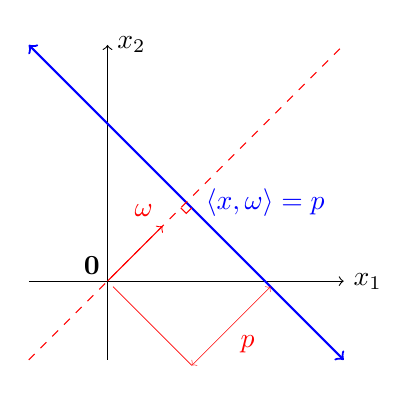
\begin{tikzpicture}[plane/.style={<->,thick,blue},
        vector/.style={->,red},
        axis/.style={->,black}]
    %draw axes
    \draw[axis] (-1,0) -- (3,0) node[anchor=west]{$x_1$};
    \node at (-.2,.2) {$\mathbf{0}$};
    \draw[axis] (0,-1) -- (0,3) node[anchor=west]{$x_2$};
    %draw plane
    \draw[plane] (-1, 3) -- (3, -1) node[midway, right]{~$\langle x, \omega\rangle = p$};
    %draw projection angle and orthogonal vector
    \draw[red,dashed] (-1,-1) -- (3,3);
    \def\ra{.07};
    \draw[red] (1-\ra, 1-\ra) -- (1,1-2*\ra) -- (1+\ra,1-\ra);
    \draw[vector] (0,0) -- (0.7,0.7) node[above left]{$\omega$};
    %draw extension line
    \draw[very thin, red] (\ra, -\ra) -- (1+\ra, -1-\ra);
    \draw[<->,very thin, red] (1+\ra, -1-\ra) -- (2+\ra, -\ra) node[midway,below right]{$p$};
  \end{tikzpicture}
  \caption{Hyperplane equation}\label{fig:HypEq}
\end{figure}

Unless otherwise indicated all measures are Euclidean measures — that is the Borel measure associated with the standard Euclidean metric on a given region of integration. In particular the Euclidean measure on a hyperplane of $\RR^n$ is equivalent to the Euclidean measure on $\RR^{n-1}$. We choose for convenience to denote measures by their associated variable such as $dx$, $dp$, $dz$, and others. It should be stated that this notation, while uniform, is context dependent. For example in the integrals
\[
  \int_{\RR^n}~dx \qquad \text{and} \qquad \int_{\langle x, \omega\rangle = p} ~dx,
\]
the measure $dx$ is to be understood as the $n$-dimensional and $(n-1)$-dimensional Euclidean measure respectively.

\section{Classical and multivariate moment problems}
% Let $f(x)$ be a measurable function on $\RR$. For $k \in \NN_0$, define the $k$th moment of $f$ as
% \[
%   c_k = \int_{-\infty}^\infty f(x)x^k ~dx.
% \]
% The sequence ${(c_k)}_{k \in \NN_0}$ is called a moment sequence or a moment problem, and the function $f$ is called a solution to the moment problem. Loosely speaking a moment problem poses the question: Under given constraints (e.g.\ domain, continuity, etc\ldots), to what extent can one determine the solution $f$ from its moments?
Let $\mu$ be a Borel measure on $\RR$. For $k \in \NN_0$, define the $k$th moment of $\mu$ as
\[
  c_k = \int_{-\infty}^\infty x^k ~d\mu(x)
\]
provided the integral converges. The sequence ${(c_k)}_{k \in \NN_0}$ is called a moment sequence or a moment problem, and the measure $\mu$ is called a solution to the moment problem. Loosely speaking a moment problem poses the question: Under given constraints (e.g.\ measures supported within a fixed subset of $\RR^n$), to what extent can one determine a solution $\mu$ (if one exists) from a moment sequence? 

The classical study of moment problems is divided into three cases depending on the support of $\mu$. In each case there is a standard choice of support, from which general results are often derived by a change of variables.
\begin{enumerate}[label=]
  \item \emph{Markov} (or \emph{Haussdorf}) moment problems within a bounded support.
  \[
    \text{supp}(\mu) \subseteq [0,1]
  \]
  \item \emph{Stieltjes} moment problems within a one-sided infinite support. 
  \[
    \text{supp}(\mu) \subseteq [0,\infty)
  \]
  \item \emph{Hamburger} moment problems within a two-sided infinite support.
  \[
    \text{supp}(\mu) \subseteq \RR
  \]
\end{enumerate}

In some special cases we will denote the moments $c_k$ in a particular form:
\begin{enumerate}
  \item When $\mu$ is absolutely continuous with respect to the Lebesgue measure $dx$, moments can be defined by
  \[
    c_k = \int f(x)x^k dx
  \]
  where $f(x)$ is the density of $\mu$ with respect to $dx$.
  \item When $\mu$ is the Lebesgue measure on a set $A$ of finite measure, moments can be defined by
  \[
    c_k = \int_A x^k dx.
  \]
\end{enumerate}
We often use these representations interchangeably. For example, we may say a function $f$ is determinate, or a set $A$ is indeterminate, if the corresponding measure $\mu$ has that property.

There are two natural questions one can ask about a moment problem:
\begin{itemize}[label=]
  \item \emph{Solvability}: Does a solution $\mu$ exist possessing the given moments?
  \item \emph{Determinacy}: Is a solution unique? If not, what can be said about the set of solutions?
\end{itemize}

For our purposes we will assume existence. In terms of the shape reconstruction method of Chapter 3 it is taken as a given that a solution exists, but that we have access only to the moments. Furthermore in practical application we encounter a followup question to determinacy: How can we reconstruct the solution?

In the classical cases (Markov, Stieltjes, Hamburger) these questions have been more or less resolved. Precise conditions for solvable and determinate moment problems have been found, and the nature of solution sets to indeterminate moment problems are well understood. For instance, all solvable Markov moment problems are unique. This result follows from the Weierstrass approximation theorem:

\begin{proposition}
  All Markov moment problems are determinate. If $\mu, \nu$ are Borel measures on the unit interval $[0,1]$ with equal moments,
  \[
    \int_0^1 x^k d\mu = \int_0^1 x^k d\nu, \qquad k \in \NN_0,
  \]
  then $\mu = \nu$.
\end{proposition}

% \begin{proof}
%   By linearity it is sufficient to show that if $c_k = 0$ for all $k \in \NN_0$, then $\mu = 0$. Furthermore, 
% \end{proof}

\begin{myexample}
  An example of an indeterminate Stieltjes moment problem?
\end{myexample}

However, in the case of multivariate moment problems remain largely open. Let $\mu$ be a Borel measure now on $\RR^n$. For $\alpha \in \NN_0^n$. Define the $\alpha$th multivariate moment of $f$ as 
\[
  c_\alpha = \int_{\RR^n} x^\alpha ~d\mu(x).
\]

\begin{myexample}
  Let $A = {[0,1]}^n \subseteq \RR^n$ be the unit cube and $\mu$ the Lebesgue measure on $A$. Then $\mu$ has multivariate moments
  \begin{align*}
    \int_{\RR^n} x^\alpha ~d\mu(x) 
    &= \int_{{[0,1]}^n} x_1^{\alpha_1}x_2^{\alpha_2} \cdots x_n^{\alpha_n} dx \\
    % &= \int_0^1 \int_0^1 \cdots \int_0^1 x_1^{\alpha_1}x_2^{\alpha_2} \cdots x_n^{\alpha_n} ~dx_1~dx_2\cdots~dx_n \\
    &= \int_0^1 x_1^{\alpha_1} ~dx_1 \int_0^1 x_2^{\alpha_2} ~dx_2 \cdots \int_0^1 x_n^{\alpha_n} ~dx_n \\
    &= \frac{1}{(\alpha_1+1) (\alpha_2+1) \cdots (\alpha_n+1)}
  \end{align*}
  Similarly the Lebesgue measure $\mu$ on any rectanglular region $A = \prod_{i = 1}^n [a_i, b_i]$ has moments
  \[
    \int_A x^\alpha ~d\mu(x) 
    = \prod_{i=1}^n \int_{a_i}^{b_i} x_i^{\alpha_i} ~dx_i
    = \prod_{i = 1}^n \frac{b_i^{\alpha_i + 1} - a_i^{\alpha_i + 1}}{\alpha_i + 1}
  \]
\end{myexample}
The moment sequence ${(c_\alpha)}_{\alpha \in \NN_0^n}$ is now multi-indexed, but the notions of solvability and determinacy are analogous: It is solvable provided there exists a Borel measure with these moments, and it is determinate provided such a measure is unique. Here, we divide multivariate moment problems into two cases:

\begin{enumerate}[label=]
  \item \emph{Bounded} multivariate moment problems within a bounded support.
  \[
    \text{supp}(\mu) \subseteq {[0,1]}^n
  \]
  % \item \emph{Stieltjes} multivatiate moment problems within a half-plane. 
  % \[
  %   \text{supp}(\mu) \subseteq \RR^{n-1} \times [0, \infty)
  % \]
  \item \emph{Unbounded} multivariate moment problems within an unbounded support.
  \[
    \text{supp}(\mu) \subseteq \RR^n
  \]
\end{enumerate}

While conditions for the solvability or determinacy of multivariate moment problems have been found in certain cases \cn, they are nowhere near as comprehensive as those of classical moment problems. One straightforward, albeit limited, approach is to reduce and $n$-variate moment problem to a set of $n$ univariate moment problems~\cite{Pete82}. For example, we employ this strategy in our proofs of propositions [determinacy for bounded domain and gaussian measures].

As in the classical case of Markov moment problems, determinacy is a consequence of Stone-Weierstrass ($n$-variate polynomials):
\begin{proposition}
  If $\mu$ is a Borel measure on the unit cube $A = {[0,1]}^n$, with moments
  \[
    c_\alpha = \int_{A} x^\alpha d\mu, \qquad \alpha \in \NN_0^n
  \]
  then the moment problem $(c_\alpha)_{\alpha \in \NN_0^n}$ is determinate.
\end{proposition}
We present a simple alternate proof in section 1.4 via the Radon transform.

\begin{myexample}
  An example of an indeterminate, unbounded, multivariate moment problem?
\end{myexample}

\section{Gaussian measures and the Hermite polynomials}
We review the definitions of univariate and multivariate Gaussian measures and Hermite polynomials, and discuss some basic properties. An extensive investigation of Gaussian measures can be found in [Bogachev] \cn. The univariate Hermite polynomials are well known, but there are multiple multivariate generalizations. We use a simple product definition.

First we review some basic properties of the univariate Gaussian measure.

\begin{definition}
  Let $w(p) : \RR \rightarrow \RR$  be the standard Gaussian density on $\RR$,
  \[
    w(p) = \frac1{\sqrt{2\pi}} e^{\frac{-p^2}2}
  \]
  and $w_n(x) : \RR^n \rightarrow \RR$ the standard Gaussian density on $\RR^n$,
  \[
    w_n(x) = {(2\pi)}^{-\frac n2} e^{\frac{-\|x\|^2}2}.
  \]
  Note that $w = w_1$.
\end{definition}

A couple of formulas: First the Gaussian integral,
\[
  \int_{-\infty}^\infty w(p) ~dp = 1.
\]
This can be proven in a number of clever ways.

\begin{proof}
  We would like to show that 
  \[
    \int_{-\infty}^\infty e^{-\frac{p^2}2} dp = \sqrt{2\pi}
  \]
  % \[
  %   \int_{\RR^n} e^{-\frac{\norm{x}^2}2} dx = {(2\pi)}^{-\frac{n}2}
  % \]
  \pn
\end{proof}
Second: The derivative
\[
  w'(p) = -pw(p).
\]

Third: The Gaussian function dominates polynomials in the sense that
\[
  \lim_{p \rightarrow -\infty} P(p)w(p) = 0 = \lim_{p \rightarrow \infty} P(p)w(p)
\]
for any polynomial $P$.

\begin{definition}
  The \textit{Gaussian moments} of a function $f: \RR^n \rightarrow \RR$ are
  \[
    c^G_\alpha = \int_{\RR^n} f(x)x^\alpha w(x) ~dx
  \]
  for $\alpha \in \NN_0^n$.
\end{definition}

\begin{myexample}
  Let $f: \RR \rightarrow \RR$ be the constant function $f(p)=1$. The Gaussian moments of $f$, i.e.\ the moments of $w(p)$, are
  \[
    c^G_k 
    = \begin{cases}
        (k-1)!!, & k~\text{even} \\
        0, & k~\text{odd}
    \end{cases}
  \]
  We have already seen $c_0 = 1$. Furthermore it is not hard to see that for odd $k$, 
  \[
    c^G_k = \int_{-\infty}^\infty p^k w(p) ~dp = 0
  \]
  since $p^k w(p)$ is an odd function.

  Now for $\ell = 1, 2, \ldots$, we derive a recurrence formula for $c_{2\ell}$ by integrating by parts
  \begin{align*}
    c^G_{2\ell}
    &= \int_{-\infty}^\infty p^{2\ell} w(p) ~dp \\
    &= -\int_{-\infty}^\infty p^{2\ell-1} \left(-p w(p)\right) ~dp \\
    &= - \left[p^{2\ell-1} w(p)\right]_{-\infty}^\infty + (2\ell-1)\int_{-\infty}^\infty p^{2\ell-2} w(p) ~dp \\
    &= (2\ell-1)c^G_{2\ell-2}.
  \end{align*}
  Thus by induction,
  \[
    c^G_{2\ell} = (2\ell - 1)(2\ell - 3) \cdots c_0 = (2\ell-1)!!.
  \]

  As an alternate derivation, for readers familiar with the gamma function $\Gamma(z) = \int_0^\infty t^{z-1}e^{-t}$ we present the following. Since $p^{2\ell} w(p)$ is even,
  \begin{align*}
    \int_{-\infty}^\infty p^{2\ell} e^{-\frac{p^2}2} dp 
      &= 2\int_0^\infty p^{2\ell} e^{-\frac{p^2}2} dp 
  \end{align*}
  Now substituting $t = \frac{p^2}2$, whereby $dt = p~dp$,
  \begin{align*}
    2\int_0^\infty p^{2\ell} e^{-\frac{p^2}2} dp 
      % &= 2\int_0^\infty p^{2\ell - 1} e^{-\frac{p^2}2} dt \\
      &= 2^{\ell+\frac12}\int_0^\infty t^{\ell - \frac12}e^{-t} dt \\
      &= 2^{\ell+\frac12} \Gamma\left(\ell + \frac12\right)
  \end{align*}
  so that
  \[
    c^G_{2\ell} = \frac{2^{\ell}}{\sqrt{\pi}} \Gamma\left(\ell + \frac12\right) = (2\ell - 1)!!
  \]
\end{myexample}



A relationship between the univariate and multivariate Gaussian densities can be seen as follows: Let $x, y \in \RR^n$, $n \geq 2$. Suppose $y = p\omega$ where $\omega \in S^{n-1}$ and $p \in \RR$, so that $p\omega$ is the orthogonal projection of $x$ onto the span of $y$. Then the Pythagorean relation,
\[
  \|x\|^2 = \|x - p\omega\|^2 + \|p\omega\|^2 = \|x - p\omega\|^2 + p^2
\]
implies that
\begin{align*}
  w_n(x) 
  &= {(2\pi)}^{-\frac n2} e^{\frac{-\|x\|^2}2} \\
  &= {(2\pi)}^{-\frac{n-1}2} e^{\frac{-\|x - p\omega\|^2}2} {(2\pi)}^{-\frac12} e^{\frac{-p^2}2} \\
  &= w_{n-1}(x - p\omega)w(p)
\end{align*}
The equation
\begin{equation}\label{eq:gaussPythag}
  w_n(x) = w_{n-1}(x - p\omega)w(p)
\end{equation}
is in some respect the defining property of the Gaussian measure described below. Indeed if $x = (x_1, x_2, \ldots, x_n)$, by repeated application of (\ref{eq:gaussPythag}) one can write the decomposition
\[
  w_n(x) = \prod_{k = 1}^n w(x_k).
\]
Thus the $w_n(x)$ is the product of $n$ copies of $w$. The standard Gaussian measure $\gamma^n$ is thus a measure whose cardinal projections are standard Gaussian measures.

\begin{definition}
Let $\gamma^n$ be the Borel measure on $\RR^n$ with density $w_n$,
\[
  \int_{\RR^n} f(x) d\gamma^n = \int_{\RR^n} f(x) w_n(x) ~dx.
\]
We call $\gamma^n$ the \textit{standard Gaussian measure}. 
More generally, for mean $a \in \RR^n$, and variance $\sigma > 0$, the following $\gamma^{n}_{a, \sigma^2}$ are \textit{Gaussian measures},
\begin{align*}
  \int_{\RR^n} f(x) d\gamma^n_{a,\sigma^2}
  &= \frac{{(2\pi)}^{-\frac n2}}{\sigma}  \int_{\RR^n} f(x) e^{-\frac{\|x - a\|^2}{2\sigma^2}} ~dx \\
  &= \int_{\RR^n} f(\sigma x + a) d\gamma^n
\end{align*}
% (Most general defn of Gaussian measures includes degenerate $\delta$ functions, and any product of Gaussian measures).
\end{definition}

\begin{myexample}
  Let $f:\RR^n \rightarrow \RR$ be the constant function $f(x)=1$. The Gaussian moments of $f$ are the multivariate moments of $w_n(x)$, and can be written as
  \begin{align*}
    c^G_\alpha 
    &= \int_{\RR^n} x^\alpha w_n(x) ~dx \\
    &= \prod_{i = 1}^n \int_{-\infty}^\infty x_i^{\alpha_i} w(x_i) ~dx \\
    &= \prod_{i = 1}^n c^G_{\alpha_i}
  \end{align*}
  where $\{c_k\}_{k \in \NN}$ are the univariate moments of $w(p)$.
  Thus $c^G_\alpha = 0$ if any $\alpha_i$ is odd. Otherwise, if every $\alpha_i$ is even then
  \[
    c^G_\alpha = \prod_{i = 1}^n (\alpha_i - 1)!!
  \]
\end{myexample}

% Next we discuss the Hermite polynomials. They can be defined in many equivalent ways, as orthogonal polynomials with respect to the Gaussian weight, as eigenfunctions for 

\begin{definition}
  The \emph{Hermite polynomials} can be defined by the Rodrigues formula
  \[
      H_k(p) = {(-1)}^k \frac{w^{(k)}(p)}{w(p)}
  \]
  
\end{definition}

We can derive a recurrence relation for $H_k$ with some basic differential calculus. First multiplying both sides by $(-1)^k w(p)$, we get
\[
   w^{(k)}(p) = {(-1)}^k w(p)H_k(p)
\]
Now we differentiate both sides 
\[
  w^{(k+1)}(p) 
    = {(-1)}^{k} (-pw(p)H_k(p) + w(p)H_k'(p)) 
    = {(-1)}^{k+1} w(p)(pH_k(p) - H_k'(p))
\]
so that, dividing both sides by ${(-1)}^{k+1} w(p)$, we have
\[
  H_{k+1}(p) = pH_k(p) - H_k'(p)
\]
Since $H_0(p)$ is trivially the constant $1$ we compute the first handful of polynomials:
\begin{align*}
  H_0(p) &= 1 \\
  H_1(p) &= p \\
  H_2(p) &= p^2 - 1 \\
  H_3(p) &= p^3 - 3p \\
  H_4(p) &= p^4 - 6p^2 + 3 \\
  H_5(p) &= p^5 - 10p^3 + 15p
\end{align*}
Note that each $H_k$ is a monic polynomial of  degree $k$, and $H_k$ is an even (odd resp.) function if $k$ is even (odd resp.).
The Hermite polynomials are mutually orthogonal in the sense that for nonnegative integers $\ell < k$,
\begin{align}\label{eq:HOrth}
  \int_{-\infty}^\infty H_\ell(p) H_k(p) w(p)~dp 
  = 0
\end{align}
To see this, substitute the Rodrigues formula for $H_k$,
\[
  (-1)^k \int_{-\infty}^\infty H_\ell(p) w^{(k)}(p)~dp
\]
and integrate by parts
\begin{align*}
  (-1)^k \left(\left[H_k(p)w^{(k-1)}(p)\right]_{-\infty}^\infty - \int_{-\infty}^\infty H'_\ell(p) w^{(k-1)}(p)~dp\right) \\
  = (-1)^{k-1}\int_{-\infty}^\infty H'_\ell(p) w^{(k-1)}(p)
\end{align*}
where the boundary term $\left[H_k(p)w^{(k-1)}(p)\right]_{-\infty}^\infty$ vanishes because of $w(p)$'s rapid decay at $\pm \infty$. Repeat this process until $H_\ell$ is annihilated.

% \begin{remark}
%   We describe (\ref{eq:HOrth}) in terms of ``orthogonality'' because 
% \end{remark}

The Hermite polynomials form a complete orthogonal basis for $L^2(\RR, w)$, the space of function $f : \RR \to \RR$ for which $\int_{-\infty}^\infty f(p)^2 w(p)~dp < \infty$. This is a Hilbert space with inner product $\langle f, g \rangle = \int_{-\infty}^\infty |f(p)g(p)| w(p)~dp$.
\begin{proposition}
   The linear span of the Hermite polynomials $H_0(p), H_1(p), \ldots$ is dense in $L^2(\RR, w)$.
\end{proposition}

\begin{corollary}
  For any $f \in L^2(\RR)$ the moment problem given by
  \[
    c_n = \int_{-\infty}^\infty f(p) w(p) dp
  \]
  is determinate.
\end{corollary}

In the section 1.5 we will make use of a different definition for the Hermite polynomials, as Taylor series coefficients for an exponential generating function.
\begin{lemma}
  The Hermite polynomials have the \emph{generating function},
  \[
    \phi(p) = e^{pt - \frac{t^2}2} 
      = \sum_{k = 0}^\infty \frac{H_k(p)}{k!}t^k.
  \]
  which converges absolutely for all $p, t \in \RR$.
\end{lemma}

\begin{proof}
Note that
\[
  e^{pt - \frac{t^2}2} 
    = \frac{e^{-\frac{(p-t)^2}2}}{e^{-\frac{p^2}2}} 
    = \frac{w(p - t)}{w(p)}
\]
so that the Taylor coefficients are precisely
\[
  \left[\frac{d^k}{dt^k}\frac{w(p - t)}{w(p)}\right]_{t = 0} 
    = (-1)^k \frac{w^{(k)}(p)}{w(p)} = H_k(p).
\]
\end{proof}

We can now define a straight forward multivariate analogue or the 
Hermite polynomials 

\begin{definition}
  For $\alpha \in \NN_0^n$ we define the \emph{multivariate Hermite polynomial} $H_\alpha$ by
\[
  H_{\alpha}(x) = H_{\alpha_1}(x_1) \cdots H_{\alpha_n}(x_n), \qquad x = (x_1, \ldots x_n) \in \RR^n 
\]
\end{definition}

The multivariate Hermite polynomials have many useful properties corresponding to those of the classical polynomials. In particular we have the Rodrigues formula
\[
  H_\alpha(x) 
    = (-1)^{|\alpha|}\frac{\partial^{\alpha}w_n(x)}{w_n(x)}
\]
where $\partial^\alpha = \frac{\partial^{\alpha_1 + \cdots + \alpha_n}}{\partial x_1^{\alpha_1} \cdots \partial x_n^{\alpha_n}}$. Just like the classical case, this formula can be used to define $H_\alpha$ as multivariate Taylor coefficients for the generating function:
\[
  \phi(x) = e^{\langle x, y\rangle - \frac{\|y\|^2}2} 
    = \frac{w_n(x - y)}{w_n(x)} 
      = \sum_{\alpha \in \NN_0^n} \frac{H_\alpha(x)}{\alpha!}y^\alpha
\]
which we note is absolutely convergent for all $x, y \in \RR^n$. Here we use the same symbol $\phi$ for the univariate and multivariate generating functions at the risk of confusion. It should be clear from context.

% An interesting formula relating the classical and multivariate Hermite polynomials:
% \[
%   \sum_{|\alpha| = k} \frac{H_\alpha(x)}{\alpha!}y^\alpha 
%     = \frac{H_k\left(\frac{\langle x, y \rangle}{\|y\|}\right)}{k!}|y|^k
% \]
% can be found in a more general form, from Erd\'elyi, Rosier, and others \cn. If $\|y\| = 1$ this says
% \[
%   \sum_{|\alpha| = k} \frac{H_\alpha(x)}{\alpha!}y^\alpha 
%     = \frac{H_k\left(\langle x, y \rangle\right)}{k!}
% \]

% A related formula, assuming $\|y\| = 1$,
% \[
%   \sum_{|\alpha| = k} \frac{H_k(p)}{\alpha!}(y^\alpha)^2
%     = \frac{H_k(p)}{k!}
% \]
% derived independently by Sengupta, looks similar but is very different. z


\section{The Radon and Gaussian Radon transforms}

Let $f$ be a function on the $n$-dimensional Euclidean space $\RR^n$. We imagine taking ``slices'' of $f$ by restricting it to a $(n-1)$-dimensional hyperplane $\Lambda$. These hyperplanes form the domain of the Radon Transform. More precisely, the Radon Transform associates each slice with a corresponding integral
\[
  R_f(\Lambda) = \int_{\Lambda} f(x) ~dx,
\]
which can be thought of as a $(n-1)$-dimensional measurement of $f$. To be more precise we parametrize the collection of hyperplanes $\Lambda$ by normal vector, $\omega \in S^{n-1}$, and (signed) distance from the origin $-\infty < p < \infty$. Indeed any hyperplane can be described in the form $\Lambda = \{x \in \RR^n: \langle x, \omega\rangle = p\}$. As mentioned, there is a slight inconsistency in these definitions where a hyperplane $\Lambda$ can be indexed by both $\langle \omega, x \rangle = p$ and $\langle -\omega, x \rangle = -p$. This difference is inconsequential for our purposes so we choose the latter definition for clarity.

The Radon transform~\cite{Helg65} (RT) is a thing that I will discuss the history of, with references, in this paragraph. The transform gets its name from Johann Radon, whose first defined the transform in the form below in 1917, although a similar transform was introduced by Paul Funk in 1911~\cn. It is interesting to note that the primary application of the RT in medical imaging (CT scans) was not invented for another half century. I can only hope that in 2076 my dissertation will serve as an absorbent coffee coaster for a sleep deprived student.

\begin{definition}
  Let $f$ be a nonnegative measurable function on $\mathbb{R}^n$. The \emph{Radon transform} $R_f : S^{n-1} \times \RR \rightarrow \RR$ of $f$ is a function which, given a unit vector $\omega \in \RR^n$ and $p \in \RR$, is defined as
  \[
    R_f(\omega, p) = \int\mclimits_{\langle x, \omega \rangle = p} f(x) ~dx,
  \]
  provided the integral converges.
\end{definition}

\begin{myexample}
  For computation it is convenient to write the Radon Transform with an explicit isometric parameterization $x(t)$ of the hyperplane $\langle x, \omega\rangle = p$. In particular we note that there exists a map $x : \RR^{n-1} \rightarrow \RR^n$ such that $x(0) = p\omega$ and
  \[
    R_f(\omega, p) = \int_{\RR^{n-1}} f(x(t)) dt.
  \]

  For reference let's specify an hyperplane parameterization for the $n=2$ case. In $\RR^2$ often we identify $\omega$ with the angle $0 \leq \theta < 2\pi$ such that $\omega = (\cos \theta, \sin \theta)$. We define $x(t)$ by
  \begin{align*}
    x(t) = (t \sin \theta + p \cos \theta, -t \cos \theta + p \sin \theta), \qquad -\infty < t < \infty.
  \end{align*}
  It is not difficult to show that $x(0) = p\omega$, $\langle x(t), \omega \rangle = p$, and most importantly
  \[
    R_f(\omega, p) = \int_{-\infty}^\infty f(t \sin \theta + p \cos \theta, -t \cos \theta + p \sin \theta)~dt
  \]
\end{myexample}

\begin{myexample}
  Let $B(r) = \{x : |x| \leq r\} \subseteq \RR^n$ be the ball of radius $r$.
  \[
    R_{B(r)}(\omega, p) = 
    \begin{cases}
      V_{n-1}\left(\sqrt{r^2 - p^2}\right), & |p| \leq r \\
      0 & |p| > r
    \end{cases}    
  \]
  where $V_n(r)$ is the volume of a hypersphere of radius $r$,
  \[
    V_n(r) = \frac{\pi^{n/2}}{\Gamma(\frac n2+1)} r^n.
  \]
  Note that as a bounded domain, we can guarantee $B(r)$ is integrable on all hyperplanes. In fact the RT of any subset of $B(r)$ is sharply bounded by $R_{B(r)} \leq V_{n-1}(r)$. Also note that $B(r)$ is rotation invariant, hence $R_{B(r)}(\omega, p)$ is independent of $\omega$.
  
  \begin{figure}[h]
    \centering
    \includegraphics[width=0.7\textwidth]{Images/Ball RT.png}
    \caption{The RT of a ball}\label{fig:RTBall}
  \end{figure}

  We can use this formula to determine the RT of an annulus. Let $A(r_1, r_2) = \{x \in \RR^n: r_1 \leq \|x\| \leq r_2\}$. Then
  \begin{align*}
    R_{A(r_1, r_2)}(\omega, p) 
    &= R_{B(r_2)}(\omega, p) - R_{B(r_1)}(\omega, p) \\
    &= 
    \begin{cases}
      V_{n-1}(\sqrt{r_2^2 - p^2}) - V_{n-1}(\sqrt{r_1^2 - p^2}), & |p| < r_1 \\
      V_{n-1}(\sqrt{r_2^2 - p^2}), & r_1 \leq |p| \leq r_2 \\
      0, & |p| \geq r_2
    \end{cases}
  \end{align*}
\end{myexample}
 


Now consider an example of an unbounded region.

\begin{myexample}
Let $S = \{(x,y) : |y| \leq \frac12\} \subseteq \RR^2$ be a strip centered on the $x$-axis with width $1$. Clearly if $\theta = \pi/2$ or $3\pi/2$ then 
\[
  R_S(\theta, p) = 
  \begin{cases}
      \infty, & |p| \leq \frac12 \\
      0, & |p| > \frac12
  \end{cases}.
\]
Otherwise, 
\[
  R_S(\theta, p) = \sec \theta
\]
Note because $S$ is unbounded, that $R_S$ is not only unbounded, but even divergent in some cases.

\begin{figure}[h]
  \centering
  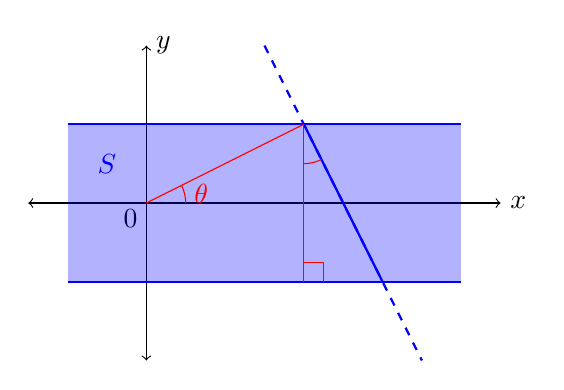
\begin{tikzpicture}[strip/.style={blue, fill=blue, fill opacity = 0.3},
      angle/.style={red},
      axis/.style={<->,black}]
  %draw axes
  \draw[axis] (-1.5,0) -- (4.5,0) node[anchor=west]{$x$};
  \node at (-.2,-.2) {$0$};
  \draw[axis] (0,-2) -- (0,2) node[anchor=west]{$y$};
  %draw wedge
  \fill[strip] (-1, 1) -- (4,1) -- (4, -1) -- (-1, -1) -- cycle;
  \draw[thick, blue] (-1,1) -- (4,1);
  \draw[thick, blue] (-1,-1) -- (4,-1);
  \node[blue] at (-0.5,0.5) {$S$};
  %draw hyperplane
  \draw[thick, blue, dashed] (1.5,2) -- (3.5,-2);
  \draw[thick, blue] (2,1) -- (3,-1);
  %draw angles
  \def\ra{.5};
  \draw[red] (0,0) -- (2,1);
  \draw[red] (\ra,0) arc (0:26.57:\ra) node[midway, right]{$\theta$};
  \draw[red] (2,1) -- (2,-1);
  \draw[red] (2,-1+\ra/2) -- (2+\ra/2,-1+\ra/2) -- (2+\ra/2,-1);
  \draw[red] (2,1-\ra) arc (270:296.57:\ra);
  % \draw[red] (-1,0) arc (180:135:1)node[midway, left]{$\delta$};
  \end{tikzpicture}
  \caption{RT of a strip}\label{fig:strip}
\end{figure}
% More generally, if $S(\varphi, r_1, r_2) = \{(x,y) : r_1 \leq x \cos \varphi + y \sin \varphi \leq r_2\}$ is a strip then (I'm guessing here)
% \[
%     R_{S(\varphi, r_1, r_2)} =
%     \begin{cases}
%         (r_2 - r_1) \sec (\theta - \varphi), & \theta \neq \varphi \pm \frac\pi2 \\
%         \infty, & \theta = \varphi \pm \frac\pi2 \text{ and } p \in [r_1, r_2] \\
%         0, & \theta = \varphi \pm \frac\pi2 \text{ and } p \not\in [r_1,r_2]
%     \end{cases}
% \]
\end{myexample}

Our main addition to previous work will be the use of a modified RT, the Gaussian Radon transform (GRT). This transform is very similar to the RT, but the inclusion of a Gaussian density $w_{n-1}(x)$ in the integral allows for convergence on a larger class of functions $f$. This includes for example unbounded regions. In a broader context the Gaussian Radon transform also has the advantages of generalizing to infinite dimensional Hilbert spaces~\cite{Seng14} (on which the Lebesgue measure is not defined), as well as having a natural probabilistic interpretation.

\begin{definition}
The \textit{Gaussian Radon transform} $GR_f : S^{n-1} \times \RR \rightarrow \RR$ of $f$ is defined similarly to the RT.\@ Given $\omega \in S^{n-1}$ and $-\infty < p < \infty$, the GRT is
\[
  GR_f(\omega, p) = 
  \int\mclimits_{\langle x, \omega \rangle = p} f(x) w_{n-1}(x - p\omega) ~dx.
\]
provided the integral converges. Note the Gaussian density 
\[
  w_{n-1}(x - p\omega) = {(2\pi)}^{-(n-1)/2}e^{-\|x - p\omega\|^2/2}
\] 
is centered on the point of the hyperplane closest to the origin.
\end{definition}

\begin{figure}[h]
    \centering
    \includegraphics[width=0.7\textwidth]{Images/GRT.png}
    \caption{The GRT}\label{fig:GRT}
\end{figure}

\begin{remark}
  It may be helpful to understand the GRT as a simple modification of the RT with respect to a Gaussian measure on $\RR^n$. From the relation
  \begin{align*}
    \int\mclimits_{\langle x, \omega \rangle = p} f(x) w_n(x) ~dx
    &= \int\mclimits_{\langle x, \omega \rangle = p} f(x) w_{n-1}(x) ~dx~ w(p),
  \end{align*}
  we can express the GRT of $f$ in terms of the $RT$ of the function $g(x) = f(x)w_n(x)$:
  \begin{equation}
    \label{eq:GRTPythag}
    R_g(\omega, p) = GR_f(\omega, p) w(p), \qquad g(x) := f(x)w_n(x).
  \end{equation}
  The relation above provides decent intuition for the GRT, and is also a useful tool proving some basic properties of the transform. Expand on intuition (maybe with example.)
\end{remark}

\begin{myexample}
  If $x(t):\RR^{n-1} \to \RR^n$ is a parametrization of $\langle x, \omega\rangle = p$ as described above, then
  \[
    GR_f(\omega, p) = \int_{\RR^{n-1}}f(x(t)) w_{n-1}(t) dt
  \]
  In particular for $f:\RR^2 \to \RR$
  \[
    GR_f(\omega, p) = \int_{-\infty}^\infty f(t \sin \theta + p \cos \theta, -t \cos \theta + p \sin \theta) w(t)~dt
  \]
  where $\omega = (\cos \theta, \sin \theta)$.
\end{myexample}

\begin{myexample}
  The Gaussian Radon transform is bounded for any measurable region $A \subseteq \RR^n$. Indeed 
  \[
      GR_A(\omega, p) \leq GR_1(\omega, p) = \int_{\RR^{n-1}} w_{n-1}(t)dt w(p) = w(p)
  \]
\end{myexample}

\begin{myexample}
  Consider the Strip $S \subseteq \RR^2$ from [earlier example]. While the RT of $S$ was divergent for $\theta = \pi/2$ or $3\pi/2$, the GRT converges. In particular,
  \[
    GR_S(\theta, p)
    = \begin{cases}
      \frac1{\sqrt{2\pi}}e^{-\frac{p^2}2}, & |p| \leq \frac12 \\
      0, & |p| > \frac12
    \end{cases}
  \]
  This is the density of a ``truncated'' normal distribution on $[-\frac12,\frac12]$. For other angles $GR_S(\theta, p)$ is likewise the density of a truncated normal distribution, this time with arbitrary endpoints $[a, b]$, given by
  \[
    a = ?, \qquad b = a + \sec\theta
  \]
\end{myexample}

Now imagine sweeping a hyperplanar ``slice'' across $\RR^n$. As a function of $p$, $R(\omega, p)$ can be seen as a projection of $f$ onto the linear subspace spanned by $\omega$. It is not surprising that integrating this projection over $-\infty < p < \infty$ we get the same result as the $n$-fold integral of $f$ over $\RR^n$.
\[
    \int_{-\infty}^\infty R(\omega, p) ~dp = \int_{\RR^n} f(x) ~dx
\]
The so called ``slice theorem'' further generalizes this observation:

\begin{proposition}[Slice Theorem]
  % If $f: \RR^n \rightarrow \RR$ and $F: \RR \rightarrow \RR$ are measureable, then
  If $f \in L^1(\RR^n)$ and $F \in L^\infty(\RR)$, then
  % If $f \in C_c(\RR^n)$ and $F \in L^1_{loc}(\RR)$, then
  % \needed{EXTRA CONDITIONS} (i.e. non-negative Fubnini,  Tonelli)
  \begin{align}
    \label{eq:ST}
    \int_{-\infty}^\infty R_f(\omega, p) F(p) dp 
    % &= \int_{-\infty}^\infty \int_{\langle x, \omega \rangle = p} f(x) F(p) ~d\mu(x) ~dp 
    &= \int_{\mathbb{R}^n} f(x) F(\langle x, \omega \rangle) dx,
  \end{align}
  % so long as one of the two is finite.
\end{proposition}

\begin{proof}
  This is a corollary of the Fubini-Tonelli theorem, which guarantees the slice formula as the integrals on either side converge absolutely. To see this note that there is a rigid transformation (Hilbert space isomorphism) taking this to an iterated integral over $\RR^{n-1}$ and $\RR$. Further, $F(\langle x, \omega \rangle) \in L^\infty(\RR^n)$, so the proposition follows by H\"older's inequality
  \[
    \int_{\RR^n} \left|f(x) F(\langle x, \omega \rangle)\right| ~dx \leq \int_{\RR^n}|f(x)| ~dx \|F(\langle x, \omega \rangle)\|_\infty <  \infty
  \] 
  % (under which the Euclidean measures are invariant), the is an integral over $\RR^{n-1}$
  % Fubini's theorem applies since if 
  % Inserting the definition of the RT, the left side is
  % \[
  %   \int_{-\infty}^\infty \int\mclimits_{\langle x, \omega \rangle = p} f(x) ~dx~ F(p) ~dp 
  %   = \int_{-\infty}^\infty \int\mclimits_{\langle x, \omega \rangle = p} f(x) F(\langle x, \omega \rangle) ~dx dp.
  % \]
  % Up to a rigid transformation (under which the Euclidean measures are invariant) this is essentially an iterated integral over $\RR$ and $\RR^{n-1}$. Thus given the integrability requirement, Fubini's theorem applies and the slice theorem is proved.
\end{proof}

\begin{remark}
  % Although we invoke the general Fubini condition here, we note a couple of more convenient sufficient conditions. First, if $f \in L^1(\RR^n)$ and $F \in L^\infty(\RR)$ then,
  The sufficient conditions for the slice theorem above can loosened significantly. We can take for example the straightforward Fubini condition 
  \[
      \int_{\RR^n} |f(x)F(\langle x, \omega \rangle )| < \infty
  \]
  which is necessary \cn, but not convenient. We may also use the condition $f$ has bounded support and $F \in L^1_{loc}(\RR)$.

  The conditions on $f$ and $F$ can be reduced somewhat. In general the convergence of either the left or right side above is sufficient. One 
  % We can specify various conditions for convergence. If $F(p)$ is bounded then $\int |f(x)| dx < \infty$ suffices for convergence. If $f$ is continuous with compact support then $F(p)$ only needs to be integrable.  
\end{remark}

If $F(p) = e^{-ip}$ and $f(x)$ is such that $\int_{-\infty}^\infty R_f(\omega, p) dp < \infty$ then (\ref{eq:ST}) becomes the well known Fourier slice theorem
\[
  \int_{-\infty}^\infty R_f(\omega, p) e^{-ip} ~dp
  = \int_{\mathbb{R}^n} f(x) e^{-i\langle x, \omega\rangle} ~dx,
\]
which is often articulated as saying that the $1$-dimensional Fourier transform of the Radon transform is the $n$-dimensional Fourier transform of $f$.

An early and natural question in the study of the RT is that of inversion. Radon himself derived the ``Radon inversion formula''~\cite{Rado17}~\cite{Rado86}, which is often proved via the above Fourier slice theorem. The groundbreaking inversion formula is the basis for what, in application, called ``filtered back-propagation''.

If one is interested in inverting the RT then a prerequisite concern is of course: Is the transform injective? The answer clearly depends on what space we draw the function $f$ from. Radon~\cite{Rado17}~\cite{Rado86} provides a set of sufficient regularity conditions such that the RT is invertible. Other similar results followed \cite{????}. On the other hand counterexamples have been constructed by, for example, Lawrence Zalcman~\cite{Zalc82}, of continuous and nontrivial functions for which the RT is identically zero.

By way of the relation (\ref{eq:GRTPythag}) we can prove an analogous slice theorem for the GRT.\@ Mihai and Sengupta prove the general result if real, separable, infinite Hilbert spaces \cn.

\begin{proposition}[Gaussian Slice Theorem] 
  Let $f:\RR^n \rightarrow \RR$ and $F:\RR \rightarrow \RR$ be measurable functions. If $f \in L^1(\RR^n, w_n)$ and $F \in L^\infty(\RR)$ then
  \begin{equation}\label{eq:GST}
    \int_{-\infty}^\infty GR_f(\omega, p)F(p) w(p) ~dp
    = \int_{\mathbb{R}^n}f(x) F(\langle x, \omega\rangle) w_n(x) ~dx. 
  \end{equation}
\end{proposition}

\begin{remark}
  Again the more general Fubini condition
  \[
    \int_{\mathbb{R}^n} |f(x) F(\langle x, \omega\rangle) w_n(x)| dx < \infty
  \]
  may be used. Further, whatever conditions on $f$ and $F$ are sufficient for convergence in (\ref{eq:ST}) are then sufficient conditions to be checked of $f(x)w_n(x)$ and $F(p)w(p)$. I'll need to check these conditions more carefully.
\end{remark}



\begin{proof}
  From (\ref{eq:GRTPythag})
  \[
    \int_{-\infty}^\infty GR_f(\omega, p)F(p) w(p) ~dp 
    = \int_{-\infty}^\infty R_g(\omega, p) F(p) ~dp
  \]
  where $g(x) = f(x)e^{-\|x\|^2/2}$. Note that $\|g\|_1 = \|f\|_{1,w_n} < \infty$ and. Then applying the slice theorem:
  \[
    \int_{-\infty}^\infty R_g(\omega, p) F(p) ~dp 
    = \int_{\RR^n} f(x)F(\langle x, \omega \rangle) w_n(x) ~dx,
  \]
  completing the proof.
\end{proof}

% \begin{remark}
%     For an equivalent 
% \end{remark}

\section{The Radon transform of measures}

% Here we extend the definitions of the RT and GRT to apply to 

Taking from the context of classical moment problems we should define the notion of the Radon transform of a measure $\mu$. Let $\mu$ be a Borel measure on $\RR^n$ with finite moments $c_\alpha$, $\alpha \in \NN_0^n$. The projection $\pi_\omega : \RR^n \rightarrow \RR$ given by
\[
  \pi_\omega(x) = \langle x, \omega \rangle
\] 
is a Borel function, thus we may define the push-forward measure $\mu_\omega = \mu \circ \pi_\omega^{-1}$ which for Borel sets $A \subseteq \RR$ is given by,
\[
  \mu_\omega(A) = \mu(\pi_\omega^{-1}(A)) = \mu(\{x : \langle x, \omega \rangle \in A\}).
\]
We may call $\mu_\omega$ the \emph{marginal projection measure} of $\mu$ with direction vector $\omega$.

Notice that if $\mu$ is absolutely continuous with density representation $\mu = f(x)dx$ then the slice theorem with $F(p)$ the characteristic function of $A$ gives,
\[
  \mu(\pi_\omega^{-1}(A)) = \int\mclimits_{\langle x, \omega \rangle \in A} f(x)dx = \int_A R_f(\omega, p) dp
\]
so that in fact $\mu_\omega$ is absolutely continuous with respect to the Lebesgue measure $dp$ and it's density is precisely the Radon transform $R_f(\omega, p)$. In this sense the marginal projection $\mu_\omega$ is a natural generalization of the RT, so we define

\begin{definition}
  The Radon transform of a Borel measure $\mu$ on $\RR$ is defined as the push-forward measure $\mu_\omega = \mu \circ \pi_\omega^{-1}$ on $\RR$, where $\pi_\omega: \RR^n \rightarrow \RR$ is the projection 
  \[
    \pi_\omega(x) = \langle x, \omega \rangle.
  \]
  We may denote this measure by $R_\mu^\omega = \mu_\omega$.
\end{definition}

\begin{remark}
  It seems that the slice theorem is analogous to — and perhaps generalized by — the change of variables formula for the push-forward measure $R^\omega_\mu$:
  \[
    \int_{-\infty}^\infty F(p) dR^\omega_\mu(p) = \int_{\RR^n} F(\pi_\omega(x)) d\mu
  \]
  where $F:\RR \rightarrow \RR$ is integrable with respect to $dR^\omega_\mu$ if and only if $F\circ\pi_\omega : \RR^n \rightarrow \RR$ is integrable with respect to $\mu$.
\end{remark}
Can we similarly define the GRT of a measure?

\begin{proposition}
  Let $c_\alpha (\omega) = \int_{-\infty}^\infty R_f(\omega, p) p^k dp$ be the projection moments of $f$ at a fixed $\omega$, and $c_\alpha$ the multivariate moments of $f$. Then
  \[
      c_k(\omega) = \sum_{|\alpha| = k}\binom{k}{\alpha} \omega^\alpha c_\alpha
  \]
  where $\binom{k}{\alpha} = \frac{k!}{\alpha_1! \alpha_2! \cdots \alpha_n!}$ are multinomial coefficients.
\end{proposition}

\begin{proof}
  By the slice theorem (\ref{eq:ST}) with $F(p) = p^k$,
  \[
    \int_{-\infty}^\infty R_f(\omega, p) p^k ~dp 
    = \int_{\RR^n} f(x) \langle x, \omega \rangle^k ~dx.
  \]
  Now $\langle x, \omega \rangle^k = {(x_1 \omega_1 + \cdots + x_n \omega_n)}^k$ has the multinomial expansion
  \[
    \langle x, \omega \rangle^k = \sum_{|\alpha| = k}\binom{k}{\alpha} x^\alpha\omega^\alpha.
  \]
  Thus after a bit of rearranging we get
  \begin{align*}
    \int_{\RR^n} f(x) \langle x, \omega \rangle^k ~dx
    &= \int_{\RR^n} f(x) \sum_{|\alpha| = k}\binom{k}{\alpha} x^\alpha \omega^\alpha ~dx \\
    &= \sum_{|\alpha| = k}\binom{k}{\alpha} \omega^\alpha \int_{\RR^n} f(x) x^\alpha ~dx,
  \end{align*}
  where the integrands are precisely the $k$th degree multivariate moments of $f$.
\end{proof}

Similarly, moments of the GRT (Gaussian projection moments) can be expressed in terms of multivariate gaussian moments.

\begin{proposition}
  Let $c_k^G(\omega) = \int_{-\infty}^\infty GR_f(\omega, p) p^k w(p) dp$ be the Gaussian moments of the GRT of $f$ at a fixed $\omega$. Let $c^G_\alpha = \int_{\RR^n} f(x) w_n(x) x^\alpha dx$ be the Gaussian multivariate moments of $f$. Then
  \[
    c^G_k(\omega) = \sum_{|\alpha| = k}\binom{k}{\alpha} \omega^\alpha c^G_\alpha.
  \]
\end{proposition}


\begin{proof}
  The proof follows as it did for the RT.\@ This time we apply the GRT slice theorem (\ref{eq:GST}) with $F(p) = p^k$, 
  \begin{align*}
    \int_{-\infty}^\infty GR_f(\omega, p) p^k w(p) ~dp
    &= \int_{\RR^n} f(x) \langle x, \omega \rangle^k w_n(x) ~dx
  \end{align*}
  Again we use the multinomial expansion of $\langle x, \omega\rangle^n$ and rearrange:
  \[
    \int_{\RR^n} f(x) \langle x, \omega \rangle^k w_n(x) ~dx
    = \sum_{|\alpha| = k} \binom{k}{\alpha} \omega^\alpha \int_{\RR^n} f(x) w_n(x)x^\alpha dx. 
  \]
  Thus
  \[
    c^G(\omega) = \sum_{|\alpha| = k} \binom{k}{\alpha} \omega^\alpha c^G_\alpha.
  \]
\end{proof}

\begin{myexample}
  Let $e_1, e_2, \ldots, e_n \in S^{n-1}$ be the the standard basis for $\RR^n$,
  \[
    (1, 0, \ldots, 0),~ (0, 1, \ldots, 0),~ \ldots,~ (0,0, \ldots, 1)
  \]
  Then $\langle x, e_i \rangle = x_i$ is the natural projection of $\RR^n$ onto the $e_i$ axis. The standard projection moments can be calculated as follows
  \begin{align*}
    c_k(e_i) 
    &= \sum_{|\alpha| = k} \binom{k}{\alpha} e_i^\alpha c_\alpha \\
    &= c_{ke_i}
  \end{align*}
  since $e_i^\alpha = 0$ unless $\alpha = ke_i$.
\end{myexample}

The following theorem, due to Petersen \cn, gives a way us to reduce the question of determinacy for multivariate moment problems to the classical case.

\begin{proposition}[Petersen's theorem]
  Let $\mu$ be a Borel measure with finite moments on $\RR^n$, and $e_1, \ldots, e_n$ the standard basis for $\RR^n$. If each $R_\mu^{e_1}, \ldots, R_\mu^{e_n}$ is determinate, then $\mu$ is determinate.
\end{proposition}

\begin{proof}
  An outline of the proof is as follows. Preliminarily, note that the solution set $[\mu]$ of Borel measures with equivalent moments to $\mu$ is convex \cn, and a $\mu$ is an extreme point in $[\mu]$ if and only if polynomials are dense in $L^1(\RR^n, \mu)$ \cn. Thus it suffices to show that polynomials are dense in $L^1(\RR^n, \mu')$ for any $\mu' \in [\mu]$.
  
  The family of products of continuous functions of compact support $f(x) = \prod_{i=1}^n f_i(x_i)$ where each $f_i \in C_c(\RR)$, is dense in $L_1(\mu)$ \cn. Furthermore, since $R_\mu^{e_i}$, $i = 1, \ldots, n$ are determinate, polynomials are dense in each $L^2(\RR, R_\mu^{e_i})$ \cn. Petersen constructs a series of polynomials $P_i : \RR \rightarrow \RR$ such that the polynomial product $P(x) = \prod_{i = 1}^n P_i(x_i)$ arbitrarily close to $f$ in $L^1(\mu)$. Thus polynomials are dense in $L^1(\RR^n, \mu)$ and the moment problem is determinate. \pn 
  
  Note Schm\"udgen proves this via Borel characteristic functions. Not clear what the benefit is.
\end{proof}

\begin{remark}
  Conjecture? We expect this result to hold true for any orthonormal basis, and likely any basis. Will have to check this. Arguable benefit for us is that we in theory can use any $n$ linearly independent projections to reconstruct $\mu$.
\end{remark}

\begin{corollary}
  If $\mu$ is compactly supported Borel measure on $\RR^n$, then the multivariate moment problem is determinate.
\end{corollary}

\begin{proof}
  It suffices to note that the projections $R_\mu^{e_i}$ are compactly supported Borel measures on $\RR$, and thus determinate by \cn.
\end{proof}


We show in section (2.2) that any function $f$ in the weighted space $L^2(\RR, \gamma)$ is determinate (maybe this should be moved to section 1.2). Petersen's theorem allows us to generalize this result to $\RR^n$.

\begin{corollary}
  If $f \in L^2(\RR^n, \gamma^n)$, then $f$ is determinate.
\end{corollary}

\begin{proof}
  % This follows from the product decomposition of the the Gaussian density
  % \[
  %   w_n(x) = \prod_{i = 1}^n w(x_i)
  % \]
  % so that
  % \[
  %   R_f(e_i, p) = \int_{x_i=p} f(x) w_n(x) dx
  % \]
  \pn
\end{proof}

\section{The Radon transform of multivariate Hermite polynomials over general affine subspaces}

% The goal of this section will be to explore the generalizations of the RT and GRT as functions of general affine subspaces. We discuss the analogues of many of the previous results in this context.
We begin this section by proving a formula for the GRT of the multivariate Hermite polynomials defined in the previous section. Recall that for $\alpha \in \NN_0^n$ the polynomials $H_\alpha(x)$ can be defined by the generating function
\[
  e^{\langle x, y\rangle - \frac{\|y\|^2}2} = \sum_{\alpha \in \NN_0^n} \frac{H_\alpha(x)}{\alpha!} y^\alpha
\]
where $\alpha! = \alpha_1! \cdots \alpha_n!$. These are related to the classical Hermite polynomials by
\[
  H_\alpha(x) = \prod_{i=1}^n H_{\alpha_i}(x_i)
\]
where, for $k \in \NN_0^\infty$, the classical polynomials $H_{k}(p)$ can be defined by
\[
  e^{pt - \frac{t^2}2} = \sum_{k = 0}^\infty \frac{H_k(p)}{k!}t^k.
\]

\begin{proposition} \label{prop:GRTHermite}
  Let $\omega \in S^{n-1}$ and $p \in \RR$ be fixed. If $|\alpha| = k$, then the GRT of the multivariate Hermite polynomial $H_\alpha$ is
  \begin{equation}\label{eq:GRH}
    GR_{H_\alpha}(\omega, p) = H_k(p)\omega^\alpha
  \end{equation}
\end{proposition}

\begin{proof}
  Recall that the generating function $\phi(x) = e^{\langle x, y\rangle - \frac{\|y\|^2}2}$ converges absolutely for all $x,y \in \RR^n$. Consider the GRT of $\phi$,
  \begin{align*}
    GR_{\phi}(\omega, p) 
      &= \int\mclimits_{\langle x, \omega \rangle = p} \phi(x) w_{n-1}(x - p\omega)~dx.
    % \\&= \int\mclimits_{\langle x, \omega \rangle = 0} \phi(x + p\omega) w_{n-1}(x)~dx
  \end{align*}
  Immediately we can expand $\phi(x)$, interchanging integral and series, to see
  \begin{equation} \label{eq:GRTPhiExpansion1}
    \begin{split}
      GR_{\phi}(\omega, p)
        &= \sum_{\alpha \in \NN_0^n} \frac1{\alpha!} y^\alpha \int\mclimits_{\langle x, \omega\rangle = p} H_\alpha(x) w_{n-1}(x - p\omega)~dx
      \\&= \sum_{\alpha \in \NN_0^n} \frac{GR_{H_\alpha}(\omega, p)}{\alpha!} y^\alpha.
    \end{split}
  \end{equation}
  On the other hand, we will be able to show that
  \begin{equation} \label{eq:GRTPhiExpansion2}
    GR_{\phi}(\omega, p) 
    = \sum_{k = 0}^\infty \sum_{|\alpha| = k} \frac{H_k(p)\omega^\alpha}{\alpha!} y^\alpha.
  \end{equation}
  Thus, being careful to note that the series (\ref{eq:GRTPhiExpansion1}) and (\ref{eq:GRTPhiExpansion2}) converge absolutely, we can compare coefficients for the desired formula. In order to derive the second expansion we begin by translating our integral onto the linear subspace $\langle x, \omega\rangle = 0$, via the change of variables $x \mapsto x + p\omega$:
  \begin{equation}\label{eq:GRTPhiExpansion21}
    \begin{split}
      GR_{\phi}(\omega, p) 
        &= \int\mclimits_{\langle x, \omega\rangle = 0} \phi(x + p\omega) w_{n-1}(x) ~dx 
      \\&= \int\mclimits_{\langle x, \omega\rangle = 0} e^{\langle x + p\omega, y \rangle - \frac{\|y\|^2}2}(2\pi)^{-\frac{n-1}2}e^{-\frac{\|x\|^2}2} ~dx
      \\&= e^{p \langle \omega, y\rangle - \frac{\|y\|^2}2} \int\mclimits_{\langle x, \omega\rangle = 0}e^{\langle x, y\rangle - \frac{\|x\|^2}2} (2\pi)^{-\frac{n-1}2} ~dx
    \end{split}
  \end{equation}
  Now in order to compute the right side integral we consider the orthogonal decomposition $y = y_\omega + y_{\omega^\perp}$, where
  \[
    y_\omega = \langle y, \omega \rangle \omega \qquad y_{\omega^\perp} = y - y_\omega.
  \]
  We make two observations about this decomposition of $y$: First, 
  \begin{equation}\label{eq:GRTPhiExpansion22}
    \|y\|^2 
      = \|y_\omega\|^2 + \|y_{\omega^\perp}\|^2 
      = \langle y, \omega\rangle^2 + \|y_{\omega^\perp}\|^2
  \end{equation}
  and second, for $x$ in the linear subspace $\langle x, \omega\rangle = 0$ we have
  \[
    \langle x, y \rangle
      = \langle x, \omega \rangle \langle y, \omega \rangle + \langle x, y_{\omega^\perp} \rangle 
      = \langle x, y_{\omega^\perp} \rangle.
  \]
  This second observation allows us to solve the integral at the end of (\ref{eq:GRTPhiExpansion21}). By completing the square $\|x - y_{\omega^\perp}\| = \|y_{\omega^\perp}\|^2 - 2\langle x, y_{\omega^\perp} \rangle + \|x\|^2$, we have
  \begin{align*}
    \int\mclimits_{\langle x, \omega\rangle = 0}e^{\langle x, y\rangle - \frac{\|x\|^2}2} (2\pi)^{-\frac{n-1}2} ~dx
      &= e^{-\frac{\|y_{\omega^\perp}\|^2}2} \int\mclimits_{\langle x, \omega\rangle = 0}e^{-\frac{\|y_{\omega^\perp}\|^2}2 + \langle x, y_{\omega^\perp}\rangle - \frac{\|x\|^2}2} (2\pi)^{-\frac{n-1}2} ~dx
    \\&= e^{-\frac{\|y_{\omega^\perp}\|^2}2} \int\mclimits_{\langle x, \omega\rangle = 0}e^{-\frac{\|x - y_{\omega^\perp}\|}2} (2\pi)^{-\frac{n-1}2} ~dx
    % \\&= e^{-\frac{\|p_{\omega^\perp}\|^2}2}
  \end{align*}
  which is just $e^{-\frac{\|p_{\omega^\perp}\|^2}2}$. It was important here to invoke the orthogonal projection $y_{\omega^\perp}$ so that the integrand becomes the translation of a standard Gaussian function on the hyperplane $\langle x, \omega \rangle = 0$. Now returning to (\ref{eq:GRTPhiExpansion21}), we have
  \begin{align*}
    GR_{\phi}(\omega, p) 
      &= e^{p \langle \omega, y\rangle - \frac{\|y\|^2}2-\frac{\|y_{\omega^\perp}\|^2}2}
    \\
      &= e^{p \langle \omega, y\rangle - \frac{\langle y, \omega\rangle^2}2}
  \end{align*}
  where we used (\ref{eq:GRTPhiExpansion22}). This looks like the generating function for the univariate Hermite polynomials $H_k(p)$ with $t = \langle \omega, y \rangle$, so we expand
  \begin{align*}
    GR_{\phi}(\omega, p) 
      &= \sum_{k = 0}^\infty \frac{H_k(p)}{k!} \langle \omega, y\rangle^k.
  \end{align*}
  Finally we apply the multinomial expansion of $\langle \omega, y\rangle^k$, recalling the multinomial coefficients $\binom{k}{\alpha} = \frac{k!}{\alpha!}$. Therefore
  \begin{align*}
    GR_{\phi}(\omega, p)
      &= \sum_{k = 0}^\infty \sum_{|\alpha| = k} \frac{H_k(p)}{k!} \binom{k}\alpha y^\alpha\omega^\alpha
    \\
      &= \sum_{k = 0}^\infty \sum_{|\alpha| = k} \frac{H_k(p)\omega^\alpha}{\alpha!} y^\alpha
  \end{align*}
  as needed.
\end{proof}

\begin{remark}
  The proof above was written by Dr. Sengupta. Recall that the Hermite polynomials $H_\alpha$ form a complete orthogonal basis for $L^2(\RR^n, w_n)$. In this sense the formula (\ref{eq:GRH}) completely defines the Gaussian Radon transform on this space. Indeed, it can be shown that any function $f \in L^2(\RR^n, w_n)$ has an expansion
  \[
    f(x) = \sum_{\alpha \in \NN_0^n} a^{(f)}_\alpha H_\alpha(x)
  \]
  where
  \[
    a_\alpha^{(f)} = \int_{\RR^n} f(x)H_\alpha(x) w_n(x) ~dx.
  \]
  If this expansion converges nicely on $\Lambda$ then
  \begin{align*}
    GR_f(\Lambda) 
    &= \int_\Lambda f(x) w_n(x-p_0)~dx 
    \\ 
    &= \int_\Lambda \sum_{\alpha \in \NN_0^n} a_\alpha^{(f)} H_\alpha(x) w_n(x-p_0) ~dx
    \\
    &= \sum_{\alpha \in \NN_0^n} a_\alpha^{(f)} \int_\Lambda H_\alpha(x) w_n(x-p_0) ~dx
    \\
    &= \sum_{\alpha \in \NN_0^n} a_\alpha^{(f)} GR_{H_\alpha}(\Lambda)
  \end{align*}
  If $\Lambda$ is a hyperplane $\inner{x, \omega} = p$ with $\omega \in S^{n-1}$ then this gives
  \begin{align*}
    GR_f(\Lambda) 
    &= \sum_{\alpha \in \NN_0^n} a_\alpha^{(f)} GR_{H_\alpha}(\Lambda)
    \\
    &= \sum_{\alpha \in \NN_0^n} a_\alpha^{(f)} H_{|\alpha|}(p) \omega^\alpha
    \\
    &= \sum_{k=0}^\infty H_k(p) \sum_{|\alpha| = k} a_\alpha^{(f)} \omega^\alpha
  \end{align*}
  For details on modes convergence see (Dunkl or Thangavelu) \cn. 
\end{remark}

In section 1.4 we defined the RT and GRT as the integrals of a function $f: \RR^n \rightarrow \RR$ over $n-1$ dimensional hyperplanes, the standard definitions. But there are many examples of geometric integral transforms, closely related to the hyperplane RT, which can be thought of as ``generalized Radon transforms''. In fact, the ``Funk transform'', which relates a function on the sphere $S^{3}$ to its integrals over great circles, was first introduced by Paul Funk in 1911, half a decade before Radon introduced the hyperplane RT.\. In the remainder of this chapter we discuss the notion of the RT and GRT on general $d$-dimensional affine subspaces of $\RR^n$, where $d = 0, \ldots, n$. For context, note that when $d = 1$, this is the so called ``X-ray transform'' which gets it's name from the direct application to radiology.

Let $\Lambda_0$ be a $d$-dimensional linear subspace of $\RR^n$, and $v \in \RR^n$. Then the translation of $\Lambda_0$ by $p$
\[
  \Lambda = v + \Lambda_0
\]
is called an \emph{affine subspace} of $\RR^n$. The representation above is clearly not unique since adding any member of $\Lambda_0$ to $v$ does not change $\Lambda$. However, given an affine subspace $\Lambda$ we have a canonical choice for $v$ as the closest point in $\Lambda$ to the origin. This point exists and is unique since $\Lambda$ is closed and convex. Furthermore the point $v$ defined in this way must be orthogonal to any vector in the linear subspace $\Lambda_0$. That is, $v \in \Lambda_0^\perp$, where $\Lambda_0^\perp$ is the linear subspace
\[
  \Lambda_0^\perp = \{x \in \RR^n : \langle x, y \rangle = 0 \text{ for all } y \in \Lambda\}
\]
also known as the \emph{orthogonal complement} of $\Lambda_0$. Thus we rephrase our definition as follows:

\begin{definition}
  An \emph{affine subspace} $\Lambda$ of dimension $d$ in $\RR^n$ is defined uniquely by
  \[
    \Lambda = v + \Lambda_0
  \]
  where $\Lambda_0$ is a linear subspace of dimension $d$ and $v \in \Lambda_0^\perp$. Sometimes we call $\Lambda$ a ``$d$-plane''.
\end{definition}

\begin{remark}
  Note that the hyperplanes in the original definition of the RT are $(n-1)$-planes, and the lines in the ``X-ray transform'' are $1$-planes.
\end{remark}

Recall that if $\Lambda_0$ is a fixed linear subspace of dimension $d$, the orthogonal complements $\Lambda_0^\perp$ is a linear subspace of dimension $n - d$. For any $x \in \RR^n$ there is a unique orthogonal decomposition $x = x_{\Lambda_0} + x_{\Lambda_0^\perp}$ where $x_{\Lambda_0} \in \Lambda_0$ and $x_{\Lambda_0^\perp} \in \Lambda_0^\perp$. This idea can be summarized by the expression
\[
  \RR^n = \Lambda_0 \oplus \Lambda_0^\perp.
\]

Sometimes it is convenient to have an explicit coordinate system on an affine subspace. If $u^{(1)}, \ldots, u^{(d)}$ is a orthonormal basis for $\Lambda_0$ then there is an isometric embedding of $\RR^d$ into $\RR^n$ with image $\Lambda$ given by $x(t) : \RR^d \rightarrow \Lambda$ where
\[
  x(t) = v + t_1u^{(1)} + \cdots + t_d u^{(d)}, \qquad t \in \RR^d.
\]
By this embedding can define the Euclidean measure $dx$ on $\Lambda$ as the push-forward of the Lebesgue measure on $\RR^n$, and the standard Gaussian measure on $\Lambda$ as the push-forward of $\gamma^n$. Note the $x(t)$ is defined in such a way that $x(0) = v$ which is essential when defining the Gaussian measure on $\Lambda$.

Other times we prefer not to invoke a basis-dependent isometry, and while $x(t)$ clearly depends on the choice of $u^{1}, \ldots, u^{(d)}$, we should note that the Euclidean and Gaussian measures on $\Lambda$ are independent of basis \pn.


Now we can define the natural analogue of the RT for affine subspaces, which is sometimes called the \emph{$d$-plane transform}. To be consistent with the hyperplane RT we will write $v = p\omega$, where $\omega \in S^{n-1} \cap \Lambda_o^\perp$ and $p \in \RR$. Of course this notation is unique only up to the identification $(\omega, p) = (-\omega, -p)$.

\begin{definition}
  Let $f:\RR^n \rightarrow \RR$. For any affine subspace $\Lambda = p\omega + \Lambda_0$, we define the \emph{Radon Transform of $f$ on $\Lambda$} by
  \[
    R_f(\Lambda) = \int_{\Lambda} f(x)~dx
  \]
  and the \emph{Gaussian Radon Transform of $f$ on $\Lambda$} by 
  \[
    GR_f(\Lambda) = \int_{\Lambda} f(x) w_d(x - p\omega) ~dx
  \]
  where $d$ is the dimension of $\Lambda_0$.
\end{definition}
\begin{remark}
  Explicitly, if $x(t): \RR^d \rightarrow \Lambda$ is an Euclidean isometry then 
  \[
    R_f(\Lambda) = \int_{\RR^d} f(x(t))~dt
  \]
  If furthermore $x(0) = p\omega$ then
  \[
    GR_f(\Lambda) = \int_{\RR^d} f(x(t))w(t)~dt
  \]
  However keep in mind that these definitions are independent of the particular isometry \pn.
\end{remark}

In order to generalize the formula (\ref{eq:GRH}) we begin with the integral of $H_\alpha$ over linear subspaces.

Recall that the GRT of a function $f$ over a linear subspace $\Lambda_0$ can be written
\begin{equation} \label{eq:GRRot}
  GR_f(\Lambda_0) = \int\mclimits_{\RR^d \times {\{0\}}^{n-d}} f(Rx) w_d(x) ~dx
\end{equation}
where $R \in SO(n)$ is the a rotation sending $\RR^d \subseteq \RR^n$ to $\Lambda_0$. Thus we would like to investigate the action of rotations on certain functions of interest, namely monomials and Hermite polynomials.

\begin{lemma}
  Let $f(x) = x^\alpha$ for some multi-index $\alpha \in \NN_0^n$ of degree $|\alpha| = k$. Then the rotation $f(Rx)$ has the expansion
  \begin{equation} \label{eq:monRot}
    f(Rx) = \sum_{\substack{\beta \in \NN_0^n \\ |\beta| = k}} c(R)^\alpha_\beta x^{\beta}.
  \end{equation}
  The coefficients $c(R)^\alpha_\beta$ are given by
  \[
    c(R)^\alpha_\beta 
    % = \binom{k}{\beta} \inner{P_s\bf{e}^{\otimes \beta}, \bf{e}^{\otimes \alpha}} = \sum_{i \in I(\beta)} \inner{\bf{e}_{\otimes i}, \bf{e}^{\otimes \alpha}}
    % = \sum_{i \in I(\beta)} \prod_{j = 1}^n \inner{Re_{i_j}, e_{\alpha^j}}
    = \sum_{i \in I(\beta)} \prod_{j = 1}^n \inner{Re_{i_j}, e_{\alpha^j}}
  \]
  where $\alpha^j = \ell$ if $0 < j - \alpha_1 - \cdots \alpha_{\ell - 1} \leq \alpha_\ell$ and
  \[
    I(\beta) = \{i \in \{1, \ldots, n\}^k: \hbox{$1, \ldots, n$ have multiplicity $\beta_1, \ldots \beta_n$ in $i$}\}
  \]
  Note that the inner products $\inner{Re_{i_j}, e_{\alpha^j}}$ are matrix entries for $R$. 
\end{lemma}
\begin{proof}
  First one should note that $(Rx)^\alpha$ is a homogeneous polynomial of degree $k$; a polynomial because $R$ is a linear transformation, and homogeneous because $R \in SO(n)$ so that for $\lambda \in \RR$,
  \[
    (R\lambda x)^\alpha = (\lambda Rx)^\alpha = \lambda^k (Rx^\alpha).
  \]
  Using the tensor power notation from appendix A, we can write
  \[
    (Rx)^\alpha = \prod_{i = 1}^n \inner{Rx, e_i}^{\alpha_i} = \inner{R^{\otimes k} x^{\otimes k}, \bf{e}^{\otimes \alpha}} = \inner{x^{\otimes k}, {(R^{-1})}^{\otimes k}\bf{e}^{\otimes \alpha}}
  \]
  Now we expand over the basis ${\{\bf{e}_{\otimes i}\}}_{i \in {\{1, \ldots, n\}}^k}$, noting that each tuple $i \in {\{1, \ldots, n\}}^k$ is an anagram to exactly one multiindex of degree $k$. To be precise ${\{I(\beta)\}}_{|\beta| = k}$ is a partition of ${\{1, \ldots, n\}}^k$.
  Thus 
  \begin{align*}
    \inner{x^{\otimes k}, {(R^{-1})}^{\otimes k}\bf{e}^{\otimes \alpha}}
      % &= \sum_{\substack{\beta \in \NN_0^n \\ |\beta| = k}} \sum_{i \in I(\beta)} \inner{x^{\otimes k}, (R^{-1})^{\otimes k}\bf{e}^{\otimes \alpha}} \\
      &= \sum_{\substack{\beta \in \NN_0^n \\ |\beta| = k}} \sum_{i \in I(\beta)} \inner{x^{\otimes k}, \bf{e}_{\otimes i}} \inner{\bf{e}_{\otimes i}, {(R^{-1})}^{\otimes k}\bf{e}^{\otimes \alpha}} \\
      &= \sum_{\substack{\beta \in \NN_0^n \\ |\beta| = k}} x^\beta \sum_{i \in I(\beta)} \inner{\bf{e}_{\otimes i}, {(R^{-1})}^{\otimes k}\bf{e}^{\otimes \alpha}}.
  \end{align*}
  That we have the non-tensor expression 
  \[
    \inner{\bf{e}_{\otimes i}, {(R^{-1})}^{\otimes k}\bf{e}^{\otimes \alpha}} = \prod_{j = 1}^n \inner{e_{i_j}, R^{-1}e_{\alpha^j}} = \prod_{j = 1}^n \inner{Re_{i_j}, e_{\alpha^j}}
  \]
  follows from the definition of the inner product on ${(\RR^n)}^{\otimes k}$ and further notation from appendix A.
\end{proof}
\begin{remark}
  We could write the coefficient $c(R)^\alpha_\beta$ in a slightly different form. If we define the non-decreasing tuple $\tilde{\alpha}$ associated with a multi-index $\alpha$ by
  \[
    \tilde{\alpha} = (\underbrace{1, \ldots, 1}_{\alpha_1 ~\text{times}}, \underbrace{2, \ldots, 2}_{\alpha_2 ~\text{times}}, \ldots , \underbrace{n, \ldots, n}_{\alpha_n ~\text{times}})
  \]
  then 
  \[
    c(R)^\alpha_\beta = \sum_{\sigma \in S_k} \prod_{j = 1}^n R_{\sigma \tilde{\beta}_j, \tilde{\alpha}_j}. 
  \]
  % is similar in form to the matrix determinant.
\end{remark}
\begin{myexample}
  For a simple example take the monomial $f(x) = x_1^2x_2$. Here $n = 2$, $\alpha = (2, 1)$ and $k = 3$. The partition of ${\{1, 2\}}^3$ over multi-indices $|(\beta_1, \beta_2)| = 3$ is given by
  \begin{align*}
    I(3,0) &= \{(1, 1, 1)\} \\
    I(2,1) &= \{(1, 1, 2), (1, 2, 1), (2, 1, 1)\} \\
    I(1,2) &= \{(1, 2, 2), (2, 1, 2), (2, 2, 1)\} \\
    I(0,3) &= \{(2, 2, 2)\}
  \end{align*}
  Now note that $(\alpha^1, \alpha^2, \alpha^3) = (1, 1, 2)$. If $R \in SO(2)$ is a $2 \times 2$ rotation matrix with entries $R_{i,j} = \inner{Re_i, e_j}$ then the formula (\ref{eq:monRot}) says 
  \begin{align*}
    (Rx)^\alpha 
    &= x_1^3 R_{1,1}^2 R_{1,2} \\
    &+ x_1^2x_2 \left(R_{1,1}^2R_{2,2} + 2R_{1,1}R_{2,1}R_{1,2}\right) \\
    &+ x_1x_2^2 \left(2R_{1,1}R_{2,1}R_{2,2} + R_{2,1}^2R_{1,2}\right) \\
    &+ x_2^3 R_{2,1}^2 R_{2,2}
  \end{align*}
  While tensor power notation is concise, this sort of representation is needed for computation.
\end{myexample}

\begin{proposition}
  The GRT of a monomial $f(x) = x^\alpha$ on a linear subspace $\Lambda_0$ is given by
  \[
    GR_f(\Lambda_0) = \sum_{\substack{\beta \in \NN_0^n \\ |\beta| = k}} c(R)^\alpha_\beta c^G_{\beta}
  \]
  where $c^G_\beta = \int_{\RR^d} x^\beta w_d(x) ~dx$ are the Gaussian moments on $\RR^d$. \emph{This should be indexed by only the first $d$ entries of $\beta$. Feels weird}.
\end{proposition}

\begin{proof}
  We take (\ref{eq:GRRot}),
  \[
    GR_f(\Lambda_0) = \int\mclimits_{\RR^d \times {\{0\}}^{n-d}} {(Rx)}^\alpha w_d(x) ~dx,
  \]
  and expand by (\ref{eq:monRot}),
  \begin{align*}
    \int\mclimits_{\RR^d \times {\{0\}}^{n-d}} (Rx)^\alpha w_d(x) ~dx
    &= \sum_{\substack{\beta \in \NN_0^n \\ |\beta| = k}} {c(R)}^\alpha_\beta \int_{\RR^d \times {\{0\}}^{n-d}} x^\beta w_d(x) ~dx
  \end{align*}
  as needed.
\end{proof}

\begin{proposition}
  The GRT of a multivariate Hermite polynomial $H_\alpha$ on an affine subspace $\Lambda$ is given by
  \[
    GR_{H_\alpha}(\Lambda) = \alpha! \sum_{\substack{\beta \in \NN_0^n \\ |\beta| = |\alpha|}} {c(P_{\Lambda_0^\perp})}^\beta_\alpha \frac{H_\beta(p_0)}{\beta!}
  \]
\end{proposition}

\begin{proof}
  Once again we take the GRT of the generating function $\phi(x) = e^{\inner{x, y} - \frac{\norm{y}^2}2}$, initially expanding
  \[
    GR_{\phi}(\Lambda) = \sum_{\alpha \in \NN_0^n} \frac{GR_{H_\alpha}(\Lambda)}{\alpha!} y^\alpha
  \]
  Simultaneously we have
  \begin{align*}
    GR_\phi(\Lambda) 
    &= e^{\inner{p_0, y} -\frac{\norm{y}^2}2} (2\pi)^{-\frac{d}2}\int_{\Lambda} e^{\inner{x, y} - \frac{\norm{x}^2}2}~dx \\
    &= e^{\inner{p_0, y} - \frac{\norm{y}^2}2 + \frac{\norm{P_{\Lambda_0} y}^2}2} \\
    &= e^{\inner{p_0, y} - \frac{\norm{P_{\Lambda_0^\perp} y}^2}2} \\
    &= \sum_{\alpha \in \NN_0^n} \frac{H_\alpha(p_0)}{\alpha!} {(P_{\Lambda_0^\perp} y)}^\alpha
  \end{align*}
  Now we should have noted that the formula (\ref{eq:monRot}) applies not only to rotations but to any linear transformation, so we have 
  \begin{align*}
    GR_\phi(\Lambda) 
    &= \sum_{\alpha \in \NN_0^n} \frac{H_\alpha(p_0)}{\alpha!} \sum_{\substack{\beta \in \NN_0^n \\ |\beta| = |\alpha|}} {c(P_{\Lambda_0^\perp})}^\alpha_\beta y^\beta \\
    &= \sum_{\beta \in \NN_0^n} y^\beta \sum_{\substack{\alpha \in \NN_0^n \\ |\alpha| = |\beta|}} {c(P_{\Lambda_0^\perp})}^\alpha_\beta  \frac{H_\alpha(p_0)}{\alpha!}
  \end{align*}
  Comparing coefficients we conclude.
  \[
    \frac{GR_{H_\alpha}(\Lambda)}{\alpha!} = \sum_{\substack{\beta \in \NN_0^n \\ |\beta| = |\alpha|}} {c(P_{\Lambda_0^\perp})}^\beta_\alpha \frac{H_\beta(p_0)}{\beta!}
  \]
\end{proof}

\begin{myexample}
  Let $n = 3, k = 1$
\end{myexample}


% We may note that the linear subspace $\Lambda_0$ is a rotation of $\RR^d \subseteq \RR^n$, that is there exists some $R \in SO(n)$ so that $\Lambda_0 = R(\RR^d)$. In particular
% \[
%   GR_f(\Lambda_0) = \int_{\RR^d} f(Rx)w(x)~dx.
% \]
% Since $R$ is a linear transformation $H_\alpha(Rx)$ is a polynomial of degree $|\alpha|$, it can be written in terms of the basis $H_\beta$ with $|\beta| = k$
% \[
%   H_\alpha(R(x)) = \sum_{|\beta| = k} C(R)^\alpha_\beta H_\beta(x).
% \]
% In determining the coefficients $C^\alpha_\beta(R)$ we will use the tensor product notation described in detail in appendix A. For clarity, we will write
% \[
%   x^{\otimes k} = \underbrace{x \otimes x \otimes \cdots \otimes x}_{\hbox{$k$ times}}
% \]
% and with the vector notation ${\bf e} = (e_1, \ldots, e_n) \in (\RR^n)^n$,
% \begin{align*}
%   {\bf e}_{\otimes i} &= e_{i_1} \otimes e_{i_2} \otimes \cdots \otimes e_{i_k} 
%   \\
%   {\bf e}^{\otimes \alpha}
%   &= e_1^{\otimes \alpha_1} \otimes \cdots \otimes e_n^{\otimes \alpha_n}
%   \\
%   &= \underbrace{e_1 \otimes \cdots \otimes e_n}_{\hbox{$\alpha_1$ times}} \otimes \cdots \otimes \underbrace{e_n \otimes \cdots \otimes e_n}_{\hbox{$\alpha_n$ times}}
% \end{align*}
% where $i = (i_1, \ldots i_n) \in \{1, \ldots n\}^k$ and $\alpha \in \NN_0^n$. An inner product on tensors is defined by
% \[
%   \inner{x_1 \otimes x_2 \otimes \cdots \otimes x_k,~ y_1 \otimes y_2 \otimes \cdots \otimes y_k}
%   = \inner{x_1, y_1} \inner{x_2, y_2} \cdots \inner{x_k, y_k}.
% \]  
% Thus we can express the monomial $x^\alpha$ with degree $|\alpha| = k$ as
% \[
%   x^\alpha 
%   = \prod_{i = 1}^n \inner{x, e_i}^{\alpha} 
%   = \inner{x^{\otimes k}, {\bf e}^{\otimes \alpha}}
% \]
% Since this expression is clearly independent of the particular order of the elements of ${\bf e}^{\otimes \alpha}$ we call the collection of its distinct anagrams of $I(\alpha)$. 
% % introduce the symmetrization operator
% % \[
% %   P_s(v_1 \otimes v_2 \otimes \cdots v_k) = \frac1{k!}\sum_{\sigma \in S_k} v_{\sigma^{-1}1} \otimes v_{\sigma^{-1}2} \otimes \cdots \otimes v_{\sigma^{-1}k}
% % \]
% \begin{lemma}
%   The action of a rotation $R \in SO(n)$ on the monomial $x^\alpha$ of degree $|\alpha| = k$ has the expansion
%   \[
%     (Rx)^\alpha = \sum_{|\beta| = k} x^{\alpha} \binom{k}{\beta} \sum_{i \in I(\alpha)} \inner{e_{\otimes i}, (R^{-1})^{\otimes k}{\bf e}^{\otimes \alpha}}
%   \]
% \end{lemma}
% Now consider the action of a rotation $R \in SO(n)$ on the monomial. First it should be noted that $(Rx)^\alpha$ is a polynomial, since $R$ is a linear transformation. Furthermore for any scalar $\lambda$ we have
% \[
%   (R(\lambda x))^\alpha = (\lambda Rx)^\alpha = \lambda^k (Rx)^\alpha
% \]
% so that it is remains homogeneous polynomial of degree $k$. Now introducing the tensor notation above we have
% \begin{align*}
%   (Rx)^\alpha 
%   &= \inner{(Rx)^{\otimes k}, {\bf e}^{\otimes \alpha}}
%   \\
%   &= \inner{R^{\otimes k} x^{\otimes k}, {\bf e}^{\otimes \alpha}}
%   \\
%   &= \inner{x^{\otimes k}, (R^{-1})^{\otimes k}{\bf e}^{\otimes \alpha}}
%   \\
%   &= \inner{x^{\otimes k}, (R^{-1}{\bf e})^{\otimes \alpha}}
% \end{align*}
% where we use the shorthand $R^{-1}{\bf e} = (R^{-1}e_1, \ldots, R^{-1}e_n)$. Now recall that $\{e_{i_1} \otimes e_{i_2} \otimes \cdots \otimes e_{i_k} : (i_1, \ldots, i_k) \in I^k\}$ where $I = \{1, \ldots n\}$ is a basis for the vector space $(\RR^n)^{\otimes k}$ of $k$-tensors, so that
% \[
%   \inner{x^{\otimes k}, (R^{-1}{\bf e})^{\otimes \alpha}} 
%   = \sum_{(i_1, \ldots, i_k) \in I^k} \inner{x^{\otimes k}, e_{i_1} \otimes \cdots \otimes e_{i_k}}\inner{e_{i_1} \otimes \cdots \otimes e_{i_k}, (R^{-1}{\bf e})^{\otimes \alpha}}
% \]


% Let's take a moment to investigate the coefficients in this expansion. Take for an example $n = 3$, $k = 6$, $\alpha = (2, 1, 3)$, $\beta = (2, 2, 2)$. The tensors ${\bf e}^\beta$ and $(R^{-1}{\bf e})^{\alpha}$ are 
% \begin{align*}
%   {\bf e}^\beta &= &e_1 &\otimes &e_1 &\otimes &e_2 &\otimes &e_2 &\otimes &e_3 &\otimes &e_3
%   \\
%   (R^{-1}{\bf e})^{\alpha} &= &R^{-1}e_1 &\otimes &R^{-1}e_1 &\otimes &R^{-1}e_2 &\otimes &R^{-1}e_3 &\otimes &R^{-1}e_3 &\otimes &R^{-1}e_3
% \end{align*}
% which gives the itemwise inner product
% \begin{align*}
%   \inner{{\bf e}^{\otimes \beta}, (R^{-1}{\bf e})^{\otimes \alpha}} 
%     &= &\inner{e_1, R^{-1}e_1} \inner{e_1, R^{-1}e_1} \inner{e_2, R^{-1}e_2} 
%     \\
%     &~ &\inner{e_2, R^{-1}e_3} \inner{e_3, R^{-1}e_3} \inner{e_3, R^{-1}e_3}
% \end{align*}

% Then with $f(x) = x^\alpha$
% \begin{align*}
%   GR_f(\Lambda_0) 
%   &= \int_{\RR^d}(Rx)^\alpha w_d(x) ~dx
%   \\
%   &= \int_{\RR^d} \sum_{|\beta| = k} \inner{{\bf e}^{\otimes \beta}, (R^{-1}{\bf e})^{\otimes \alpha}} x^\beta w_d(x) ~dx
%   \\
%   &= \sum_{|\beta| = k} \inner{{\bf e}^{\otimes \beta}, (R^{-1}{\bf e})^{\otimes \alpha}} \int_{\RR^d}x^\beta w_d(x) ~dx
%   \\
%   &= \sum_{|\beta| = k} \inner{{\bf e}^{\otimes \beta}, (R^{-1}{\bf e})^{\otimes \alpha}} c^G_\beta
% \end{align*}
% where $c^G_\beta$ are the Gaussian moments on $\RR^d$
% \[
%   c^G_\beta 
%   = \int_{\RR^d} x^\beta w_d(x) ~dx 
%   = 
%   \begin{cases}
%     \prod_{i = 1}^n (\beta_\ell - 1)!! & \hbox{every $\beta_i$ even} \\
%     0 & \hbox{any $\beta_i$ odd}
%   \end{cases}
% \]

% Once again taking the generating function $\phi(x) = e^{\inner{x,y} - \frac{\norm{y}^2}2}$, we have
% \[
%   GR_\phi(\Lambda_0) 
%   = \int_{\RR^d} e^{\inner{Rx,y} - \frac{\norm{y}^2}2}
%   = \int_{\RR^d} e^{\inner{x,R^{-1}y} - \frac{\norm{R^{-1}y}^2}2}
%   = \sum_{\alpha \in \NN_0^n} \frac{H}
% \]

% In order to generalize the formula (\ref{eq:GRH}) to the general extended GRT setting it is useful to begin with a discussion of rotations of monomials. Suppose $R \in O(n)$, that is $R : \RR^n \to \RR^n$ is a linear isomorphism satisfying
% \[
%   R^\top R = RR^\top = I
% \]
% Since a linear subspace $\Lambda_0$ of dimension $d = 0, \ldots, n$ can be written as $R(\RR^d)$ for some $R \in O(n)$, and thus the affine subspace $\Lambda = p\omega + \Lambda_0$ as
% \[
%   \Lambda = p\omega + R(\Lambda_0),
% \]
% we can redefine the RT and GRT correspondingly. In particular,
% \[
%   GR_f(\Lambda) = \int_{\RR^d} f(p\omega + R^{-1}x)w(x)~dx
% \]
% For monomials $f(x) = x^\alpha$, $\alpha \in \NN_0^n$, we have
% \begin{align*}
%   f(R^{-1}x) 
%     &= (R^{-1}x)^\alpha
%     \\ 
%     &= (\sum_{i = 1}^n \inner{R^{-1}x, e_i})e_i)^\alpha
%     \\
%     &= \prod_{i = 1}^n \inner{R^{-1}x, e_i}^{\alpha_i}
%     \\
%     &= \prod_{i = 1}^n \inner{x, Re_i}^{\alpha_i}
% \end{align*}




% To illustrate the calculation of a GRT with an explicit isometry, let
% \[
%   f(x) = e^{\langle x, y\rangle}
% \]
% for some $y \in \RR$. Suppose $\Lambda = p\omega + \Lambda_0$ is a $d$-dimensional affine subspace, where $\Lambda$ is a linear subspace, $\omega \in \Lambda_0^\perp$, $y \in \RR$, and let $x(t) : \RR^d \rightarrow \Lambda$ be the isometry given by
% \[
%   x(t) = p\omega + \sum_{i = 1}^d t_iu^{(i)}
% \]
% where $u^{(1)}, \ldots, u^{(d)}$ is an orthonormal basis for $\Lambda_0$. Furthermore let $y = y_{\Lambda_0} + y_{\Lambda_0^\perp}$ and note that $\langle x, y \rangle = \langle x, y_{\Lambda_0}\rangle$ for $x \in \Lambda_0$. Then
% \begin{align*}
%   GR_f(\Lambda) 
%     &= \int_{\RR^d} e^{\langle x(t), y \rangle} (2\pi)^{-\frac{d}2} e^{-\frac{\|t\|^2}2}~dt
%   \\
%     &= e^{p \langle \omega, y \rangle} \int_{\RR^d} e^{\sum_{i = 1}^d t_i\langle u^{(i)}, y_{\Lambda_0}\rangle - \frac{\|t\|^2}2} (2\pi)^{-\frac{d}2} ~dt
%   \\
%     &= e^{p \langle \omega, y \rangle} \int_{-\infty}^\infty \prod_{i=1}^d e^{t_i\langle u^{(i)}, y_{\Lambda_0}\rangle - \frac{t_i^2}2} (2\pi)^{-\frac12} dt_i
% \end{align*}
% Now notice in each exponential in the product we can complete the square $\|t_iu^{(i)} - y_{\Lambda_0}\|^2 = \|y_{\Lambda_0}\|^2 - 2t_i\langle u^{(i)}, y_{\Lambda_0}\rangle + t_i^2$, that is
% \[
%   e^{t_i\langle u^{(i)}, y_{\Lambda_0}\rangle - \frac{t_i^2}2}
%     = e^{\frac12\|y_{\Lambda_0^\perp}\|}e^{-\frac12\|t_iu^{(i)} - y_{\Lambda_0}\|^2}
% \]
% for $i = 1, \ldots, d$. The right hand integral is a Gaussian integral equal to $1$. Thus
% \[
%   GR_f(\Lambda) = e^{p \langle \omega, y \rangle} \prod_{i=1}^d 
% \]

% Let's see if we can derive a formula for the GRT of the multivariate Hermite polynomials on a general affine plane.

% Following the proof for the hyperplane GRT, we begin again with the transform of the generating function $\phi(x)$,
% \[
%   GR_\phi(\Lambda)
%     = \int_{\Lambda_0} \phi(x) w_d(x - p\omega) ~dx
% \]
% which can be immediately expanded as 
% \[
%   GR_\phi(\Lambda) = \sum_{\alpha!}\frac{GR_{H_\alpha}(\Lambda)}{\alpha!}y^\alpha.
% \]
% At the same time we can translate the integral over to $\Lambda_0$ such that
% \[
%   GR_\phi(\Lambda)
%     = e^{p\langle \omega, y\rangle - \frac{\|y\|^2}2} \int_{\Lambda_0} e^{\langle x, y\rangle - \frac{\|x\|^2}2} (2\pi)^{-\frac d2}~dx
% \]
% As before, we decompose $y = y_{\Lambda_0} + y_{\Lambda_0^\perp}$, substitute $y_{\Lambda_0}$ for $y$ and complete the square so that the right hand integral is $e^{\frac{\|y_{\Lambda_0}\|^2}2}$.
% \[
%   GR_\phi(\Lambda) 
%     = e^{p\langle \omega, y\rangle - \frac{\|y\|^2}2 + \frac{\|P_{\Lambda_0} y\|}2}
% \]
% Now we have $\|y\|^2 = \|y_{\Lambda_0}\|^2 + \|y_{\Lambda_0^\perp}\|^2$, so
% \[
%   GR_\phi(\Lambda) 
%     = e^{p\langle \omega, y\rangle - \frac{\|y_{\Lambda_0^\perp}\|^2}2}
% \]
% Here we encounter a problem we didn't see in the hyperplane case: 
% In the hyperplane case $\dim(\Lambda_0^\perp) = 1$ so that $y_{\Lambda_0^\perp}$ was necessarily in the span of $\omega$. But for lower dimensional affine subspaces there is no immediate relation between $y_{\Lambda_0^\perp}$ and $\langle \omega, y\rangle$. 

% If we suppose for the moment that $y \in \Lambda_0^\perp$. Then we do have 
% \[
%   GR_\phi(\Lambda) 
%     = e^{p\langle \omega, y\rangle - \frac{\|y\|^2}2}
%     = \sum_{\alpha \in \NN_0^n} \frac{H_{\alpha}(p\omega)}{\alpha!}y^\alpha
% \]
% so can we conclude $GR_{H_\alpha}(\Lambda) = H_\alpha(p\omega)$? That doesn't feel right.

% If we further suppose that $y$ is in the span of $\omega$ then we find
% \[
%   something else
% \]
% via Ambar.

% What if we just assume $\|y_{\Lambda_0^\perp}\|^2 = \langle\omega, y\rangle^2$? This is true essentially if $y \in \omega\RR + \Lambda_0$. In this case we have what we want,
% \[
%   \sum_{\alpha \in \NN_0^n} \frac{GR_{H_\alpha}(\Lambda)}{\alpha!} y^\alpha = \sum_{k=0}^\infty \sum_{|\alpha| = k} \frac{H_k(p)\omega^\alpha}{\alpha!} y^\alpha
% \]
% It doesn't seem like it should be enough for this to hold on a $d+1$ subspace, to conclude that we can compare coefficients. 

% Now if $\omega$ and $P_{\Lambda_0^\perp} y$ are potentially linearly independent, where can we go from here?

% Recall $\omega$ was chosen from $S^{n-1} \cap \Lambda_0^\perp$ and $y \in \RR^n$ is arbitrary, while $P_{\Lambda_0^\perp} y$ is in $\Lambda_0^\perp$. Suppose that $v^{(1)}, \ldots, v^{(n - d)}$ is an orthonormal basis for $\Lambda_0^\perp$. We can write
% \[
%   \omega = \sum_{i = 1}^{n-d} r_i v^{(i)}, \qquad y = \sum_{i = 1}^{n-d} s_i v^{(i)}
% \]
% for some $r,s \in \RR^{n-d}$.

% Is it true that $\langle \omega, y \rangle = \langle \omega, P_{\lambda_0^\perp} y\rangle$? Well, yes: $y = P_{\Lambda_0} y + P_{\Lambda_0^\perp} y$, so
% \[
%   \langle \omega, y \rangle = \langle \omega, P_{\Lambda_0} y \rangle + \langle \omega, P_{\Lambda_0^\perp} y \rangle
% \]
% and $\langle \omega, P_{\Lambda_0} y \rangle = 0$. Then 
% \begin{align*}
%   e^{p\langle \omega, y\rangle - \frac{\|P_{\Lambda_0^\perp} y\|^2}2}
%     &= e^{p\langle \omega, P_{\Lambda_0^\perp} y \rangle - \frac{\|P_{\Lambda_0^\perp} y\|^2}2}
%   \\&= \sum_{\alpha \in \NN_0^n} \frac{H_\alpha(p\omega)}{\alpha!} (P_{\Lambda_0^\perp} y)^\alpha
%   \\&=? \sum_{\alpha \in \NN_0^{n-d}} \frac{H_\alpha(p\omega)}{\alpha!} (P_{\Lambda_0^\perp} y)^\alpha
% \end{align*}
% We still cannot compare coefficients with
% \[
%   \int_\Lambda e^{\langle x, y\rangle - \frac{\|y\|^2}2} w_{d}(x -p\omega)~dx
%     = \sum_{\alpha \in \NN_0^n} \frac{GR_{H_\alpha}(\omega, p)}{\alpha!} y^\alpha
% \]

\section{Krawtchouk polynomials}



The formula (\ref{eq:GRH}) gives us a path toward defining a discrete analogue to the Gaussian Radon transform. We will begin introducing the centered binomial density and corresponding Krawtchouk polynomials by way of a classic model in probability.

Consider flipping a loaded coin with probability $p \in [0,1]$ of landing on heads, and thus probability $(1 - p)$ of landing on tails. The probability of $k$ heads in $N$ coin flips is given by the binomial probability density,
\[
  \binom{N}{k}p^k(1-p)^{N-k}
\]
where $N \in \NN_0$ and $k = 0, 1, \ldots, N$. It is well known that the binomial distribution can be seen as a discrete analog to the Gaussian distribution. Thus we may expect that a discrete analog to the GRT may be defined via the binomial distribution.

In order to draw a clearer line between the binomial and Gaussian densities we make use of an alternate probabilistic model: the Bernoulli random walk. Picture a particle ``walking'' along the integer lattice $\ZZ$, beginning at the origin $x = 0$. At every step, we flip the loaded coin described above, stepping to the right if it lands on heads, and the left if tails. After $N$ flips, the particle's position is 
\[
  x = (\text{\# of heads}) - (\text{\# of tails}) = k - (N - k) = 2k - N
\]
Now the set of possible positions is $x \in [[N]] := \{-N, -N+2, \ldots, N\}$, and the probability of each is precisely the probability of landing $k = \frac{N + x}2$ heads, that is,
\[
  \binom{N}{\frac{N + x}2}p^{\frac{N + x}2}(1 - p)^{N - \frac{N + x}2}
  = \binom{N}{\frac{N + x}2}p^{\frac{N + x}2}(1 - p)^{\frac{N - x}2}
\]
We will define \emph{centered binomial density} supported on $[[N]]$ by
\[
  B_N(x) = \binom{N}{\frac{N+x}2}p^{\frac{N+x}2}(1-p)^{\frac{N-x}2}.
\]
Since the expected displacement at each (independent) step is $p - (1 - p) = 2p - 1$, we calculate the expected position after $N$ steps to be 
\[
  E(B_N) = 2Np-N.
\]
Furthermore the variance of each displacement step is $4p(1-p)$ so that the variance of $B_N$ is
\[
  Var(B_N) = 4Np(1-p)
\]
The earlier claim that the binomial density is a discrete analog to the Gaussian density can be made explicit by the following limit relation. Let \[
  z = \frac{x - E(B_N)}{\sqrt{Var(B_N)}} 
  = \frac{x - 2Np + N}{2\sqrt{Np(1-p)}}
\]
so that $z$ has mean $0$ and variance $1$ with respect to $B_n$. Equivalently we may set
\[
  x = z\sqrt{Var(B_N)} + E(B_N) = 2z\sqrt{Np(1-p)} + 2Np + N
\]
Then we have
\[
  \lim_{N \rightarrow \infty} B_N(x) = \frac{1}{(\sqrt{2\pi})}e^{-\frac{z^2}2} = w(z).
\]
This limit is perhaps one of the simplest cases of the robust central limit theorem, but can be proven in a number of more elementary ways \cn.

\begin{remark}
  Under an analogous limit a random walk process $x$ becomes a Brownian motion process $z$. \cn
\end{remark}

Having justified the the centered binomial densities $B_N(x)$ as discrete analogs of the Gaussian $w(z)$, we would like to define a sequence of polynomials orthogonal with respect to $B_N(x)$, as the Hermite polynomials are to $w(z)$. For convenience we start with a generating function 

\begin{definition}
  The Krawtchouk polynomials $K_k^{N,p}(x)$ may be defined by the generating function
  \[
    \sum_{k=0}^N K^{N,p}_k(x)y^k = (1 + y)^{\frac{N + x}2}(1 - y)^{\frac{N - x}2}
  \]
\end{definition}
% \begin{remark}
%   Note that this is an ordinary generating function, while that of the Hermite polynomials was a exponential generating function. Is this distinction consequential for us?
% \end{remark}

The polynomials $K^{N,p}_k(x)$ satisfy the orthogonality property
\[
  \sum_{x \in [[N]]} K^{N,p}_k(x) K^{N,p}_\ell(x) B_N(x) = 0, \qquad k \neq \ell
\]
and can be written explicitly as
\[
  K^{N,p}_k(x) = \binom{N}{k} \pFq{2}{1}{-k,(x - N)/2}{-N}{2}
\]

The Krawtchouk and Hermite polynomials are related by the same limiting process.
\begin{proposition}
  With $x = 2 z \sqrt{Np(1-p)} + 2Np + N$ we have the following limit relation:
  \[
    \lim_{N \rightarrow \infty} K^{N,p}_k(x) = H_k(z)
  \]
\end{proposition}

\begin{proof}
  \pn
\end{proof}

Now heuristically we expect a formula analagous to (\ref{eq:GRH}) in the from
\[
  GR_{K^{N,p}_\alpha}(\omega, p) = K^{N,p}_k(p)\omega^\alpha, \qquad |\alpha| = k
\]
where 
\[
  K^{N,p}_\alpha(x) = \prod_{i = 1}^n K^{N,p}_{\alpha_i}(x_i)
\]
We should resolve the conflicting variables both named $p$.

The desired formula would represent a discrete analog for the Gaussian Radon transform on the finite cubic lattice $[[N]]^n$, however it is not yet clear how to interpret this. An immediate concern is that the cubic lattice does not admit ``hyperplanes'' for arbitrary $p$ and $\omega$. Indeed in the worst case, if $\omega$ is not rational (that is the ratios between coordinates of $\omega$ are not rational, or equivalently the hyperspherical coordinates of $\omega$ include an angle which is an irrational multiple of $\pi$) then a hyperplane orthogonal can contain at most one lattice point. In the case when $\omega$ is rational — in the sense above — we may restrict $p$ to the projection of the lattice onto the span of $\omega$, and sum over the lattice hyperplane $\inner{x, \omega} = p$ with respect to the binomial weight centered on $p\omega$. It remains to be seen whether such an interpretation agrees with the heuristic formula above.

Take the symmetric random walk, where the coin is fair ($p = 1 - p = \frac12$). The position after $N$ flips has distribution
\[
  B_N(x) = \frac1{2^N}\binom{N}{\frac{N+x}2}, \qquad x \in [[N]]
\]
with expected value $E(B_N) = 0$ and variance $Var(B_N) = N$. The limiting process is then given by $B_N(x) \rightarrow w(z)$ where 
\[
  z = \frac{x}{\sqrt{N}}
\]
and further $K^{N,\frac12}_k(x) \rightarrow H_k(z)$.

Now consider the following scenario in two dimensions. A particle starting at the origin $x = (x_1, x_2) = 0$ flips two fair coins, stepping down/up depending on the first coin, left/right depending on the second. This means the particle moves one unit up and right, up and left, down and right, or down and left, with equal probability. 

\section{The Stieltjes transform}

Let $\mu$ be a Borel measure with finite moments $c_k = \int_{-\infty}^\infty p^k d\mu$. 

\begin{definition}
  The complex function $g$ defined by
  \[
    g(z) = \int_{-\infty}^\infty\frac{d\mu}{1+zp}
  \]
  is called the Markov (Hamburger resp.) transform of $\mu$ when $\mu$ has bounded (unbounded resp.) support.
\end{definition}

It is worth noting at the outset that $g(z)$ is defined at least for non-real $z$. To see this we note that if $\im z \neq 0$,
\begin{align*}
  \frac1{|1 + zp|} 
  &= \frac{|1/z|}{|\frac1z + p|} \\
  &\leq \frac{|1/z|}{|\im \frac1z|} \\
  &= \frac{|\overline{z}|/|z|^2}{|\im \overline{z}|/|z|^2} \\
  &= \frac{|z|}{|\im z|}
\end{align*}
which gives the bound
\begin{equation}
  |g(z)| 
  \leq \int_{-\infty}^\infty \frac{|z|}{|\im z|} d\mu(p) 
  = \frac{|z|}{|\im z|}c_0
\end{equation}

Since the integrand has a singularity only when $p = -1/z$ a Markov transform must converge in some neighborhood of zero. This cannot be said in general for a Hamburger transform. 

\begin{remark}
  The bound above has a useful geometric interpretation. For starters we note that,
  \[
    \frac{|\im z|}{|z|} = |\sin(\arg z)|,
  \]
  which can be seen by considering the right triangle formed by the points $0$, $z$, and $\re z$. Thus this bound essentially depends on the angle of separation between $z$ and the real line. 
\end{remark}

\begin{proposition}
  The function $g(z)$ is analytic on the upper and lower half planes $\im z \neq 0$.
\end{proposition}

\begin{proof}
  Let $z, w$ be complex numbers with non-zero imaginary part. We have
  \begin{align*}
    g(w) - g(z)
    &= \int_{-\infty}^\infty \frac{1}{1 + wp} - \frac1{1 + zp}d\mu(p) \\
    &= \int_{-\infty}^\infty \frac{(1 + zp) - (1 + wp)}{(1 + wp)(1 + zp)}d\mu(p) \\
    &= (w - z) \int_{-\infty}^\infty \frac{-p}{(1 + wp)(1 + zp)}d\mu(p).
  \end{align*}
  Thus it seems
  \[
    \lim_{w \rightarrow z} \frac{g(w) - g(z)}{w - z} = \int_{-\infty}^\infty \frac{-p}{{(1+zp)}^2}d\mu(p).
  \]
  To be precise we may justify the interchange of limit and integral here by dominated convergence. Recall that it suffices to find an integrable function $h : \RR \to \CC$ such that, for any $w$ in a neighborhood of $z$,
  \[
    \left|\frac{-p}{(1 + wp)(1 + zp)}\right| \leq h(p) \qquad \hbox{for all $p \in \RR$}.
  \]
  It should be noted that our particular dominating function $h(p)$ is somewhat arbitrary, and not a sharp bound. By the previously discussed bound we have,
  \[
    \left|\frac{-p}{(1 + wp)(1 + zp)}\right| \leq |p|\frac{|wz|}{|\im w ~\im z|}.
  \]
  Furthermore $|w|/|\im w|$ is clearly continuous on the half planes, so in some neighborhood of 
  \[
    |p|\frac{|wz|}{|\im w ~\im z|} \leq |p|\left(\frac{|z|^2}{|\im z|^2} + \epsilon\right)
  \]
  for an arbitrary $\epsilon > 0$. Finally, we note that the right hand dominating function above is integrable since $\mu$ has finite moments: 
  \[
    \int_{-\infty}^\infty |p| d\mu \leq \int_{-\infty}^\infty \frac12(p^2 + 1) ~d\mu = \frac{c_2 + c_0}2 < \infty
  \]
\end{proof}

\begin{remark}
  Since $\mu$ is a real measure, $g(z)$ commutes with conjugation,
  \[
    g(\bar z) = \int_\infty^\infty\frac{d\mu}{1+\bar zp} = \overline{\int_\infty^\infty\frac{d\mu}{1+zp}} = \overline{g(z)}.
  \]
  For this reason, although $g(z)$ is defined for all non-real $z$, we will only concern ourselves with its values on the upper half plane $\im z > 0$ going forward. In chapter 3 we should restrict our sample points to the upper half plane, since samples in the lower half may be redundant.
\end{remark}


When $z$ is a real number $g(z)$ may not converge. In particular $g(z)$ does not converge when $z = -1/p$ for some $p$ in the support of $\mu$ \pn.  Thus if $\mu$ has bounded support $g$ converges in a neighborhood of $0$. On the other hand if $\mu$ has unbounded support $g(0)$ is not defined. However — as we will see — even in the Hamburger transform case, a formal series expansion at $z = 0$ holds valuable information. The results of this section are described in detail in section 5.6 of (Baker) \cn

By a geometric series expansion,
\[
  \frac1{1 + zp} = \sum_{k = 0}^\infty {(-z)}^k p^k 
\]
when $|zp| < 1$. This suggests the connection between $g(z)$ and the moment sequence ${(c_k)}_{k \in \NN_0}$. Indeed, at least formally,
\begin{align*}
  \int_\infty^\infty\frac{d\mu}{1+zp}
  &= \int_\infty^\infty \sum_{k = 0}^\infty {(-z)}^k p^k ~d\mu \\
  &= \sum_{k = 0}^\infty {(-z)}^k \int_\infty^\infty p^k ~d\mu \\
  &= \sum_{k = 0}^\infty c_k{(-z)}^k.
\end{align*}
In the Markov case we have a positive radius of convergence. But even in the Hamburger case, there is a sense in which this asymptotic expansion holds ``non-tangentially''.

Non-tangential convergence at $z = 0$ is, as the name implies, convergence along curves not tangent to the real line at $0$. More precisely, one defines a ``wedge domain''
\[
  \Gamma_\delta = \{\delta \leq \arg z \leq \pi - \delta\}
\]
\begin{figure}
  \centering
  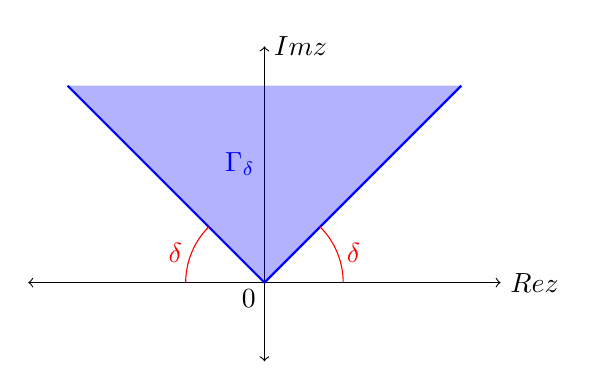
\begin{tikzpicture}[wedge/.style={blue, fill=blue, fill opacity = 0.3}, angle/.style={red}, axis/.style={<->,black}]
    %draw axes
    \draw[axis] (-3,0) -- (3,0) node[anchor=west]{$\text{Re} z$};
    \node at (-.2,-.2) {$0$};
    \draw[axis] (0,-1) -- (0,3) node[anchor=west]{$\text{Im} z$};
    %draw wedge
    \fill[wedge] (0, 0) -- (-2.5, 2.5) -- (2.5,2.5) -- cycle;
    \draw[thick, blue] (-2.5, 2.5) -- (0,0) -- (2.5,2.5);
    \node[left, blue] at (0,1.5) {$\Gamma_\delta$};
    %draw angle
    \def\ra{.07};
    \draw[red] (1,0) arc (0:45:1) node[midway, right]{$\delta$};
    \draw[red] (-1,0) arc (180:135:1)node[midway, left]{$\delta$};
  \end{tikzpicture}
  \caption{A wedge domain}\label{fig:wedge}
\end{figure}
in which curves approach $0$ with an angle at least $\delta$ from the real line.

\begin{definition} (Non-tangential convergence and asymptotic expansion)
  We say $h(z) \rightarrow 0$ non-tangentially as $z \rightarrow 0$ if, for any $\delta > 0$, the limit 
  \[
    \lim_{z \rightarrow 0} h(z) = 0
  \]
  holds for $z$ in the $\Gamma_\delta$. If a formal power series $\sum_{k=0}^\infty a_k z^k$ and a function $g(z)$ are such that for all $n\in \NN_0$,
  \[
    g(z) = \sum_{k = 0}^{n-1} c_k{(-z)}^k + z^n h_n(z)
  \]
  where the trailing terms $h_n(z)$ converge to $0$ non-tangentially as $z \rightarrow 0$, we say that $\sum_{k=0}^\infty a_k z^k$ is an asymptotic expansion of $g(z)$. We use the notation
  \[
    g(z) \simeq \sum_{k=0}^\infty a_k z^k
  \]
  for asymptotic expansions.
    % If for any $\delta > 0$ the limit $g(z) \rightarrow L$ holds 
\end{definition}

While $g(z)$ does not generally converge at $z = 0$, in a non-tangential sense the aforementioned asymptotic expansion holds:
\begin{proposition}
  \begin{enumerate}
    \item If $\mu$ has bounded support
    \[
      g(z) = \sum_{k = 0}^\infty c_k{(-z)}^k
    \]
    in a neighboorhood of $z=0$.
    \item For all $n \in \NN_0$
    \begin{equation}
      g(z) = \sum_{k = 0}^{n-1} c_k{(-z)}^k + z^n h_n(z) \label{assexp}
    \end{equation}
    where $h_n$ is such that $\lim_{z \rightarrow 0} h_n(z) = 0$ non-tangentially.
  \end{enumerate}
\end{proposition}

\begin{proof}
  We first note that 
  \[
    \sum_{k=0}^{n} c_k {(-z)}^k 
    = \sum_{k=0}^{n} \int_{-\infty}^\infty {(-zp)}^k d\mu
    % = \int_{-\infty}^\infty \sum_{k=0}^{n} (-zx)^k d\mu
    = \int_{-\infty}^\infty \frac{1 - {(-zp)}^{n+1}}{1 + zp} d\mu
  \]
  and so
  \begin{align*}
    h_n(z) = \frac1{z^n}\left\{g(z) - \sum_{k=0}^{n} c_k {(-z)}^k\right\}
    &= \int_{-\infty}^\infty \frac{zp^{n+1}}{1 + zp}d\mu.
  \end{align*}
  It remains to determine if and in what sense this trailing term $h_n(z)$ vanishes at the origin. 

  As expected in the case when $\mu$ has bounded support, $h_n(z)$ exists in a neighborhood of $0$ and vanishes as $z \rightarrow 0$ in this neighborhood. Thus the asymptotic expansion~\ref{assexp} is the Taylor expansion: The Markov transform is analytic at the origin.

  When $\mu$ has unbounded support and $h_n(z)$ may not be well defined on the real line, so we must weaken our result to non-tangential convergence. If $z \in \Gamma_\delta$ then we have the following inequalities for any $p \in \RR$,
  \[
    |p - z| \geq |p| \sin \delta 
    \quad\text{and} \quad
    |p - z| \geq |p| \sin \delta.
  \]
  We will show that
  \[
    \lim_{z \rightarrow 0} h_{2n}(z) = 0, \quad z \in \Gamma_\delta
  \]
  from which the corresponding limit for odd orders will immediately follow from the relation
  \[
    h_{2n-1}(z)
    = zh_{2n}(z) + c_{2n}z^{2n}.
  \] 
  Here for the sake of convenience we define $w = -\frac1z$, following a more classical approach. Note that $|w| = \frac1{|z|}$ and if $z$ is in the wedge $\Gamma_\delta$ then so is $w$. Now 
  \begin{align*}
    |h_{2n}(z)| 
    &\leq \int_{-\infty}^\infty \frac{|p|^{2n+1}}{|p - w|}d\mu \\
    &\leq \frac{|z|}{\sin \delta} \int_{|p| \leq A} |p|^{2n+1} d\mu
    + \frac1{\sin \delta} \int_{|p| \geq A} p^{2n} d\mu \\
    &\leq \frac{2|z| A^{2n+2}}{\sin \delta}
    + \frac1{\sin \delta} \int_{|p| \geq A} p^{2n} d\mu
  \end{align*}
  Thus 
  \[
    \lim_{z \rightarrow 0} |h_{2n}(z)| \leq \frac1{\sin \delta} \int_{|p| \geq A} p^{2n} d\mu, \quad z \in \Gamma_\delta.
  \]
  Since $A$ is arbitrary and the integral $\int p^{2n} d\mu = c_{2n}$ is convergent we are done.
\end{proof}

\begin{remark}
  An interesting connection — which I don't know enough about to discuss yet — is beginning to be revealed here between moment problems and analytic functions on the upper half plane (in particular, their behavior near the real boundary). This leads us to the notion of interpolation problems \cn.
\end{remark}

Evidently the asymptotic series expansion $g(z) \simeq \sum_{k=0}^\infty c_k {(-z)}^k$ is generally formal, having zero radius of convergence except in the Markov case. However as we will see in the next section, rational functions constructed from this formal series exist which approximate $g(z)$ on the upper half plane $\{\text{Im} z > 0\}$.

Finally we prove two propositions regarding the Hamburger transform of a RT projection. Let $\omega \in S^{n-1}$ be fixed and consider
\[
  g(z) = \int_\infty^\infty \frac{R(\omega, p)}{1 + zp} dp
\]
for some function $f: \RR^n \to \RR$. 
\begin{definition}
  The multivariate Markov (Hamburger resp.) transform of a Borel measure $\mu$ on $\RR^n$ of bounded (unbounded resp.) support is defined by
  \[
    g(y) = \int_{\RR^n} \frac{d\mu(x)}{1 + \langle x, y\rangle} \simeq \sum_{\alpha \in \NN_0^n} c_\alpha(-y)^\alpha
  \]
  when $\mu$ has finite moments $c_\alpha = \int_{\RR^n} x^\alpha d\mu$.
\end{definition}
% \begin{proposition}
%   The Hamburger transform of the Radon transform of a function $f$ is 
%   \[
%     \int_{-\infty}^\infty \frac{R_f(\omega, p)}{1 + zp} dp = \int_{\RR^n} \frac{f(x)}{1 + z\langle x, \omega \rangle} dx
%   \]
% \end{proposition}

% \begin{proposition}
  
% \end{proposition}
By applying the slice theorem, with $F(p) = {(1+zp)}^{-1}$ we see that the Hamburger transform of a projection can be represented by a similar multivariate integral of $f$ over $\RR^n$.
\[
  \int_{-\infty}^\infty \frac{R_f(\omega, p)}{1 + zp} dp = \int_{\RR^n} \frac{f(x)}{1 + z\langle x, \omega \rangle} dx
\]
Similarly the GRT slice theorem with $F(p) = {(1 + zp)}^{-1}$ is
\[
  \int_{-\infty}^\infty \frac{GR_f(\omega, p) w(p)}{1 + zp} dp = \int_{\RR^n} \frac{f(x)w_n(x)}{1 + z\langle x, \omega \rangle} dx.
\]

\section{Pad\'e approximants}

In this section we recall the necessary definitions and results. Then we will prove some new results to be applied to the Gaussian Radon transform later.

\begin{definition}[Classical definition]
  The Pad\'e approximant to a (possibly formal) power series 
  \[
    R^{[L/M]}(z) \simeq \sum_{k=0}^\infty c_k z^k
  \]
  is a rational function with numerator (denominator resp.) degree at most $L$ ($M$ resp.), with series equal to $\sum_{k=0}^N c_k z^k + O(z^{N+1})$ up to as high an order $N$ as possible. 
\end{definition}

Let
\[
  R^{[L/M]}(z) = \frac{P^{[L/M]}(z)}{Q^{[L/M]}(z)} = \frac{a_L z^L + \cdots + a_1z + a_0}{b_M z^M + \cdots + b_1z + b_0}.
\]
Notice that in general there is a negligible constant common factor between the numerator and denominator, so that with the remaining $L+M+1$ free parameters, we expect an order of accuracy of up to $L+M+1$ constraints, $c_0, c_1, \ldots, c_{L+M}$. Thus we define the $[L/M]$ Pad\'e approximant by the condition,
\begin{equation}
  \label{eq:BPade}
  \frac{P^{[L/M]}(z)}{Q^{[L/M]}(z)} = \sum_{k=0}^{L+M} c_k z^k + O\left(z^{L+M+1}\right).
\end{equation}
Multiplying by $Q^{[L/M]}(z)$ gives a necessary condition, with a subtle but important difference from (\ref{eq:BPade})
\begin{equation}
  \label{eq:CPade}
  P^{[L/M]}(z) = Q^{[L/M]}(z)\left(\sum_{k=0}^{L+M} c_k z^k\right) + O\left(z^{L+M+1}\right).
\end{equation}
In the classical theory of Pad\'e approximants (\ref{eq:CPade}) was often taken as a definition. It is always possible to find polynomials of the required degree satisfying this second condition, however they do not necessarily attain the degree of accuracy required by the first. We follow Baker, defining $R^{[L/M]}(z)$ by (\ref{eq:BPade}), provided such a rational function exists.

\begin{definition}[Baker's definition]
  The Pad\'e approximant $R^{[L/M]}$ to a (possibly formal) power series is a the unique rational function with numerator (denominator resp.) degree at most $L$ ($M$ resp.) satisfying the condition 
  (\ref{eq:BPade})
  \[
  \frac{P^{[L/M]}(z)}{Q^{[L/M]}(z)} = \sum_{k=0}^{L+M} c_k z^k + O\left(z^{L+M+1}\right).
  \] 
  If no such rational function exists we say the Pad\'e approximant does not exist.
\end{definition}

Note that the two definitions are equivalent if $b_0 = Q^{L/M}(0) \neq 0$ \pn. Hence a sufficient condition for the existence of the Pad\'e approximant by Baker's definition is that $b_0 = Q^{L/M}(0) \neq 0$. 

Equating coefficients of $z^k$, $k = 0, 1, \ldots, L+M$ in (\ref{eq:CPade}) gives two linear systems
\begin{align*}
  a_0 &= b_0c_0 \\
  a_1 &= b_1c_0 + b_0c_1 \\
  &~~\vdots \\
  a_L &= b_L c_0 + b_{L-1}c_1 + \cdots + b_0c_L
\end{align*}
and,
\begin{align*}
  0 &= b_{M}c_{L-M+1} + b_{M-1}c_{L-M+2} + \cdots + b_0c_{L+1} \\
  0 &= b_{M}c_{L-M+2} + b_{M-1}c_{L-M+3} + \cdots + b_0c_{L+2} \\
  &~~\vdots \\
  0 &= b_{M}c_L + b_{M-1}c_{L+1} + \cdots + b_0c_{L+M}
\end{align*}
where for convenience we set $c_k = 0$ for $k < 0$. The first system shows the numerator $P^{[L/M]}$ is determined by the denominator $Q^{[L/M]}$ (explicitly computing the each coefficient $a_1, \ldots, a_L$ from $b_1, \ldots b_L$). The second linear system is homogeneous, with $M$ equations in $M + 1$ unknowns. Thus we are guaranteed a nontrivial solution, and hence a Pad\'e approximant by the classical definition. A clever modification of the latter system gives us a determinantal formula for $Q^{[L/M]}$. Augmented with the desired definition, 
\[
  Q^{[L/M]}(z) = b_M z^M + b_{M-1}z^{M-1} + \cdots + b_0
\]
the system (now with dimension $M+1 \times M+1$) can be written in vector form,
\[
  \begin{pmatrix}
    0 \\ 0 \\ \vdots \\ 0 \\ Q^{[L/M]}(z)
  \end{pmatrix}
  =
  \begin{pmatrix}
    c_{L-M+1} & c_{L-M+2} & \cdots & c_{L+1} \\
    c_{L-M+2} & c_{L-M+3} & \cdots & c_{L+2} \\
    \vdots & \vdots & \ddots & \vdots \\
    c_{L} & c_{L+1} & \cdots & c_{L+M} \\
    z^M & z^{M-1} & \cdots & 1
  \end{pmatrix}
  \begin{pmatrix}
    b_M \\ b_{M-1} \\ \vdots \\ b_1 \\ b_0
  \end{pmatrix}
\]
Solving for $b_0$ by Cramer's Rule we get,
% \[
%     b_0 = 
%     \frac{
%         \left|
%         \begin{matrix}
%             c_{L-M+1} & c_{L-M+2} & \cdots & c_L & 0 \\
%             c_{L-M+2} & c_{L-M+3} & \cdots & c_{L+1} & 0 \\
%             \vdots & \vdots & \ddots & \vdots & \vdots \\
%             c_L & c_{L+1} & \cdots & c_{L+M-1} & 0 \\
%             z^M & z^{M-1} & \cdots & z & Q^{[L/M]}(z)
%         \end{matrix}
%         \right|
%     }{
%         \left|
%         \begin{matrix}
%             c_{L-M+1} & c_{L-M+2} & \cdots & c_{L+1} \\
%             c_{L-M+2} & c_{L-M+3} & \cdots & c_{L+2} \\
%             \vdots & \vdots & \ddots & \vdots \\
%             c_{L} & c_{L+1} & \cdots & c_{L+M} \\
%             z^M & z^{M-1} & \cdots & 1
%         \end{matrix}
%         \right|
%     }
% \]

% \[
%     b_0 = 
%     \frac{
%         \left|
%         \begin{matrix}
%             c_{L-M+1} & c_{L-M+2} & \cdots & c_L \\
%             c_{L-M+2} & c_{L-M+3} & \cdots & c_{L+1} \\
%             \vdots & \vdots & \ddots & \vdots  \\
%             c_L & c_{L+1} & \cdots & c_{L+M-1} 
%         \end{matrix}
%         \right| Q^{[L/M]}(z)
%     }{
%         \left|
%         \begin{matrix}
%             c_{L-M+1} & c_{L-M+2} & \cdots & c_{L+1} \\
%             c_{L-M+2} & c_{L-M+3} & \cdots & c_{L+2} \\
%             \vdots & \vdots & \ddots & \vdots \\
%             c_{L} & c_{L+1} & \cdots & c_{L+M} \\
%             z^M & z^{M-1} & \cdots & 1
%         \end{matrix}
%         \right|
%     }
% \]

\[
  b_0
  \left|
  \begin{matrix}
    c_{L-M+1} & c_{L-M+2} & \cdots & c_{L+1} \\
    c_{L-M+2} & c_{L-M+3} & \cdots & c_{L+2} \\
    \vdots & \vdots & \ddots & \vdots \\
    c_{L} & c_{L+1} & \cdots & c_{L+M} \\
    z^M & z^{M-1} & \cdots & 1
  \end{matrix}
  \right|
  =
  \left|
  \begin{matrix}
    c_{L-M+1} & c_{L-M+2} & \cdots & c_L \\
    c_{L-M+2} & c_{L-M+3} & \cdots & c_{L+1} \\
    \vdots & \vdots & \ddots & \vdots  \\
    c_L & c_{L+1} & \cdots & c_{L+M-1} 
  \end{matrix}
  \right| 
  Q^{[L/M]}(z).
\]
The LHS is a polynomial by Laplace expansion, and is nonzero if the RHS minor has nonzero determinant. Thus if the determinant
\[
  \left|
  \begin{matrix}
    c_{L-M+1} & \cdots & c_L \\
    \vdots & \ddots & \vdots  \\
    c_L & \cdots & c_{L+M-1} 
  \end{matrix}
  \right| 
\]
is nonzero, then up to the aforementioned constant factor,
\begin{equation}
  Q^{[L/M]}(z) = 
  \left|
  \begin{matrix}
    c_{L-M+1} & \cdots & c_{L+1} \\
    \vdots & \ddots & \vdots \\
    c_{L} & \cdots & c_{L+M} \\
    z^M & \cdots & 1
  \end{matrix}
  \right| 
  \label{eq:Qdet}
\end{equation}
By convention we normalize $R^{[L/M]}(z)$ so that $b_0 = Q^{[L/M]}(0) = 1$. In terms of the determinental formula above, we can write $Q^{[L/M]}(0)$ as
\[
  Q^{[L/M]}(0) = 
  \left|
  \begin{matrix}
    c_{L-M+1} & \cdots & c_{L} & c_{L+1} \\
    \vdots & \ddots & \vdots & \vdots \\
    c_{L} & \cdots & c_{L+M-1} & c_{L+M} \\
    0^M & \cdots & 0 & 1
  \end{matrix}
  \right|
  =
  \left|
  \begin{matrix}
    c_{L-M+1} & \cdots & c_{L}  \\
    \vdots & \ddots & \vdots  \\
    c_{L} & \cdots & c_{L+M-1}
  \end{matrix}
  \right|
\]
Matrices (determinants resp.) of this type — that is with antidiagonals all constant — is called a Hankel matrices (Hankel determinants resp.).  Since the Hankel determinants give a useful form for expressing some conditions of interest we will define $H(n,m)$ to be the determinant of the $(m + 1) \times (m + 1)$ Hankel matrix with $c_n, \ldots, c_{n + 2m}$ in the antidiagonals,
\[
  H(n,m) :=
  \left|
  \begin{matrix}
    c_{n} & \cdots & c_{n+m} \\
    \vdots & \ddots & \vdots  \\
    c_{n+m} & \cdots & c_{n+2m} 
  \end{matrix}
  \right|.
\]
We can relate the two previous equations by
\[
  Q^{[L/M]}(0) = H(L - M + 1, M - 1)
\]
so that the sufficient condition for the existence of $R^{[L/M]}(z)$ is $H(L-M+1, M-1) \neq 0$.

We now narrow our focus to Pad\'e approximants to a Hamburger transform. Let $\mu$ be a Borel measure on $\RR$ with finite moments $c_k = \int p^k ~d\mu$. 

With the shape reconstruction application in mind, we will now assume the measure $\mu$ is absolutely continuous with respect to the Lebesgue measure and denote it $f(x)dx$ where $f(x)$ is some non-negative Lebesgue measurable function of $\RR$. Note that by this assumption, $\mu$ cannot be supported on a finite set. The additional restriction that $\mu$ has infinite support turns out to be important when discussing the determinacy of $\mu$.

Recall that the Hamburger transform of $\mu$,
\[
    g(z) := \int_\RR \frac{d\mu}{1+pz}
\]
has the asymptotic expansion, in the sense of non-tangential limits,
\[
  g(z) \simeq \sum_{k=0}^\infty c_k (-z^k).
\]
We call this formal power series a Hamburger series. 

% \begin{remark}
%   To simplify the rest of this maybe we redefine?
%   \[
%     c_k = {(-1)}^k\int p^k d\mu
%   \]
% \end{remark}

\begin{lemma}
  The Hamburger moments $c_k$ satisfy the determinental condition $H(2n, m) \neq 0$ for $n,m = 0, 1, \ldots$. That is,
  \[
    \left|
    \begin{matrix}
      c_{2n} & \cdots & c_{2n+m} \\
      \vdots & \ddots & \vdots  \\
      c_{2n+m} & \cdots & c_{2n+2m}
    \end{matrix}
    \right| \neq 0
  \]
\end{lemma}

\begin{proof}
  
  Consider the bilinear quadratic form given by
  \[
    G(\mathbf{x}, \mathbf{y}) :=
    \mathbf{x}^\top
    \begin{pmatrix}
      c_{2n} & \cdots & c_{2n+m} \\
      \vdots & \ddots & \vdots  \\
      c_{2n+m} & \cdots & c_{2n+2m}
    \end{pmatrix}
    \mathbf{y}
  \]
  If $\mathbf{x} = {(x_0, x_1, \ldots, x_m)}^\top$ then
  \begin{align*}
    G(\mathbf{x}, \mathbf{x})
    &= \sum_{i,j=0}^m x_i x_j c_{2n+i+j} \\
    &= \sum_{i,j=0}^m x_i x_j \int p^{2n+i+j} ~d\mu \\
    &= \int \sum_{i,j=0}^m x_i x_j p^{2n+i+j} ~d\mu \\
    &= \int p^{2n} {\left(\sum_{k=0}^m x_k p^{k}\right)}^2 ~d\mu 
    \geq 0.
  \end{align*}
  Thus $G(\mathbf{x}, \mathbf{y})$ is positive semi-definite. Furthermore, equality holds
  \[
    \int p^{2n}{\left(\sum_{k=0}^m x_k p^{k}\right)}^2 ~d\mu = 0
  \]
  if and only if $\mu$ is supported entirely on the zeros of the polynomial $p^n\sum_{k=0}^m x_k p^{k}$. However by assumption $\mu$ has infinite support. So in fact $G$ is strictly positive definite. We conclude, by Sylvester's criterion for example, that associated Hankel matrix has positive determinant. That is, $H(2n, m) > 0$.
\end{proof}

The previous lemma guarantees the existence of certain Pad\'e approximants; specifically those with $L-M+1$ even. 
\begin{theorem}
  If $J$ is odd then the Pad\'e approximant $R^{[L/L+J]}(z)$ to the Hamburger series exists in Baker's sense.
\end{theorem}

% Following Baker's definition [Baker] we say the Pad\'e approximant $R^{[L/M]}$ exists if it satisfies this order of accuracy condition. For details on the construction of Pad\'e approximants see [Baker], []. When the formal series is arbitrary one cannot guarantee the existence of any given $R^{[L/M]}$. However as we will see the situation for Pad\'e approximants to a Hamburger series, for which much is known from the classical theory of moment problems and orthogonal polynomials, is much nicer than the general theory.

Let $R_M(z)$ be the ``offdiagonal'' approximant $R^{[M/M+1]}(z)$ to the Hamburger series of $\mu$,
\[
  R_M(z) = \frac{P_M(z)}{Q_M(z)} \approx \sum_{k=0}^\infty c_k {(-z)}^k \simeq \int_{-\infty}^\infty \frac{f(p)}{1 + zp} ~dp
\]
where $c_k = \int p^k f(p) dp$. In this section we will prove

\begin{theorem}
  The off-diagonal Pad\'e approximants $R_M(z)$ to the a determinate Hamburger series $\sum_{k=0}^\infty c_k {(-z)}^k$ exist and converge to $g(z)$ uniformly on compact subsets of the upper half plane $\{\text{Im} ~z > 0\}$.
\end{theorem}

An outline of the proof is as follows: We first justify that the approximants exist in Baker's sense. Then it can be shown that limit of any convergent subsequence of $R_M$ must have a representation as the Hamburger transform of some Borel measure $\mu$ which is a solution to our moment problem, and that furthermore such convergent subsequences exist. Thus in order for the sequence $R_M$ to converge to $g(z)$ it will be necessary and sufficient that the moment problem be determinate.

% Convergence $R_M(z) \rightarrow g(z)$ is \tc{related in some way cant remember} to the determinacy of the moment problem for the sequence $\{c_k\}$. Recall that a moment problem is called determinate if it has a unique solution. \tc{In Akheizer's world, if the moment problem is determinate, then $w_\infty(z)$ is a point for all $z$. Each $R_M$ coresponds to a point $w_M(\omega) = \frac1\omega R_m(-\frac1\omega)$. The points $w_M$ must converge to $w_\infty$}

\begin{proposition}
  If the sequence $c_k$ gives a determinate moment problem then the off-diagonal Pad\'e approximants $R_M(z)$ converge to $g(z)$ locally uniformly.
\end{proposition}

\begin{proof}
  The Pad\'e approximant $R_M(z)$ has a convenient representation as an inner product in terms of a finite Jacobi matrix,
  \[
    R_M(z) = \langle \delta_0, {(1 + zA_M)}^{-1} \delta_0 \rangle.
  \]
  Now since $A_M$ is a real matrix and $\frac1{|w|} \geq \frac1{|\text{Im}(w)|}$ for any $w \in \CC$, we see that
  \[
    |zR_M(z)| = |\langle \delta_0, {(z^{-1} + A_M)}^{-1} \delta_0 \rangle| \leq \frac1{|\text{Im}(1/z)|}
  \]
  and thus
  \[
    |R_M(z)| \leq \frac1{|z||\text{Im}(1/z)|} = \frac{|z|}{|\text{Im}(z)|}.
  \]
  Since this bound is independent of $R_M$, Montel's theorem implies that the off-diagonal Pade approximants form a normal family. It can be shown that the limit of any convergent subsequence has a representation $\int (1+ xz)d\sigma(x)$ where $\sigma$ is a solution to the Hamburger moment problem. Since the moment problem is determinate, the sequence $R_M$ must converge to $g(z)$ uniformly on compact sets.
\end{proof}

It remains to discuss the determinacy of the Hamburger moment problem. Here we need to add an additional constraint on the measure $d\mu = f(p)dp$, which is that $f(p)$ is $L^2$ integrable with respect to the Gaussian weight.

\begin{proposition}
  A function $f(p) \in L^2(\mathbb{R}, e^{-p^2}dp)$ such that the moments 
  \begin{equation}
    \label{eq:3}
    c_k = \int_{-\infty}^\infty p^k f(p) e^{-p^2} ~dp, ~ k = 0, 1 \ldots
  \end{equation}
  are finite, is uniquely determined by those moments.
\end{proposition}
    
\begin{proof}
  It is sufficient to show that if $c_k = 0$ for all $k \geq 0$, then $f \equiv 0$ a.e. The Hermite moments are just linear combinations of $0$,
  \[
      \int_{-\infty}^\infty H_k(p) f(p) e^{-p^2} ~dp = 0, ~ k \geq 0
  \]
  where $H_k(p)$ is the Hermite polynomial of order $k$. Since the Hermite polynomials are complete in the space $L^2(\mathbb{R}, e^{-p^2}dp)$ then $f \equiv 0$.
\end{proof}





% % \begin{figure}
% %     \centering
% %     \begin{tikzpicture}
% %         \draw[->] (0, 0) -- (5, 0) node[right] {$x$};
% %         \draw[->] (0, 0) -- (0, 1) node[above] {$y$};
% %         \draw[scale=0.5, domain=1:5, smooth, variable=\x, blue] plot ({\x}, {\x  *exp(-ln(\x))});
% %     \end{tikzpicture}
% % \end{figure}


% Given a formal power series $g(z) = \sum_{k=0}^\infty c_kz^k$ the Pad\'e approximant of degree $[L/M]$ is a rational function whose series expansion agrees with that of $g(z)$ as much as possible, which we denote by $[L/M]_g = \frac{P^{[L/M]}}{Q^{[L/M]}}$ where $P^{[L/M]}(z) = \sum_{k=0}^L a_kz^k$ and $Q^{[L/M]}(z) = \sum_{k=0}^M b_kz^k$ are polynomials of degree at most $L$ and $M$ respectively.  
% \begin{equation}
%     \label{eq:pade}
%     g(z) = [L/M]_g(z) + O(z^{N_{[L/M]}})
% \end{equation}
% Counting unknown coefficients, we can expect an order of accuracy of at most $N_{[L/M]} = L+M+1$. More precisely, we cross multiply and consider the related condition,
% \begin{equation}
%     \label{eq:cross}
%     Q^{[L/M]}(z)g(z) - P^{[L/M]}(z) = O(z^{L+M+1}),
% \end{equation}
% which can be written as a system of $L + M + 1$ linear equations
% \begin{align*}
%     \sum_{\ell = 0}^k b_\ell c_{k-\ell} &= a_k & k &= 0, 1, \ldots, L \\
%     \sum_{\ell = 0}^k b_\ell c_{k-\ell} &= 0, & k &= L + 1 \ldots, L + M
% \end{align*}
% where for convenience we set $b_\ell = 0$, $\ell > M$ and $c_\ell = 0$, $\ell < 0$. Thus a solution $b_0, \ldots, b_M$ can be found to a underdetermined homogeneous system of $M$ equations in $M+1$ unknowns, and then $a_0, \ldots, a_L$ can be computed directly. The rational function $\frac{P^{[L/M]}}{Q^{[L/M]}}$ has an irreducible form $\frac{P_\star^{[L/M]}}{Q_\star^{[L/M]}}$ which can be normalized so that $Q_\star^{[L/M]}(0) = 1$. Subject to these constraints this defines a unique rational approximation satisfying (\ref{eq:cross}) and from now the notation $[L/M]_g$ will refer to the unique normalized irreducible form $\frac{P_\star^{[L/M]}}{Q_\star^{[L/M]}}$. Note that $[L/M]_g$ computed in this way may not satisfy (\ref{eq:pade}) up to the desired order $L+M+1$, particularly in the case when $Q^{[L/M]}(0)=0$. In the event that no rational function of degree $[L/M]$ exists approximating $g$ to the desired accuracy we say the $[L/M]$ Pad\'e approximant does not exist. We will focus on cases where they do exist. Besides, in general it can be shown that infinitely many approximants exist in a sense in which we can move on to talking about convergence.

% The convergence of Pad\'e approximants is  not fully understood in general. We will concern ourselves with a particular case for which these questions have answers: approximants on a diagonal, $[m+k/m]$ as $m \rightarrow \infty$ for certain integral forms.


% Now consider the function defined by
% \[
%     g(z) = \int_{-\infty}^\infty \frac{GR_f(\omega, p)e^{-p^2}}{1 - zp} ~dp
% \]
% which has an at least formal expansion
% \[
%     g(z) \simeq \sum_{n=0}^\infty c_kz^k
% \]
% where
% \[
%     c_k = \int_{-\infty}^\infty p^k GR_f(\omega, p)e^{-p^2} ~dp.
% \]

% In this case question of the convergence $[L/M]_g \rightarrow g$ is related to whether this Hamburger moment problem is determinate.
% \begin{proposition}
% A function $f(p) \in L^2(\mathbb{R}, e^{-p^2}dp)$ such that the moments 
% \begin{equation}
%     \label{eq:3}
%     c_k = \int_{-\infty}^\infty p^k f(p) e^{-p^2} ~dp, ~ k = 0, 1 \ldots
% \end{equation}
% are finite, is uniquely determined by those moments.
% \end{proposition}

% \begin{proof}
%     It is sufficient to show that if $c_k = 0$ for all $k \geq 0$, then $f \equiv 0$ a.e. The Hermite moments are just linear combinations of $0$,
% \[
%     \int_{-\infty}^\infty H_k(p) f(p) e^{-p^2} ~dp = 0, ~ k \geq 0
% \]
% where $H_k(p)$ is the Hermite polynomial of order $k$. Since the Hermite polynomials are complete in the space $L^2(\mathbb{R}, e^{-p^2}dp)$ then $f \equiv 0$.
% \end{proof}

% \tc{My understanding here is that since the moments $c_k$ uniquely determine $GR_f(\omega, p)$, and thus $g(z)$, then the Pad\'e approximants, if they converge, must converge to $g(z)$. Correct?}


% We will now (attempt to) define a multivariate analogue to the Pad\'e approximants. We'll detail the bivariate case for example and promise that higher dimensions follow similarly. Informally, a multivariate power series is written as a sum of homogeneous polynomials, the Pad\'e approximants similarly decomposed into homogeneous polynomials. A system of linear equations is formed nearly identical to that of the classical Pad\'e approximants, but with somewhat more unknowns. A "degree shift" by $LM$ is necessary to ensure the system has a nontrivial solution. According to Cuyt the structure of this system (so called "near Toeplitz") reduces the complexity for computing solutions from $O(n^3)$ to $O(\alpha n^2)$ where $n$ is the dimension of the system and $\alpha$ is its "displacement rank." As in the univariate case it is shown these Pad\'e approximants have a unique reduced form up to a normalization constant.

% \tc{I obviously need to fill in a lot more detail here. The "degree shift" is currently what is confusing me...}

% Let me be more specific... \tc{use multi-index notation? Probably not necessary, but it looks cleaner.} Consider a formal power series in the variable $x = (x_1, \ldots, x_d) \in \mathbb{R}^d$
% \[
%     g(x) = \sum_{\alpha_1, \ldots, \alpha_d = 0}^\infty c_{\alpha_1, \ldots, \alpha_d} x_1^{\alpha_1}\cdots x_d^{\alpha_d} = \sum_{\ell = 0}^\infty C_\ell(x)
% \]
% where $C_\ell(x^\ell)$ is a homogeneous polynomial in the coordinates of $x$,
% \[
%     C_\ell(x) := \sum_{\alpha_1 + \cdots + \alpha_d = \ell} c_{\alpha_1, \ldots, \alpha_d} x_1^{\alpha_1}\cdots x_d^{\alpha_d}.
% \]
% Similarly to the univariate case we seek a rational function $[L/M]_g = \frac{P^{[L/M]}}{Q^{[L/M]}}$ where
% \[
%     P^{[L/M]}(x) 
%     % = \sum_{|\alpha| \leq L} a_\alpha x^\alpha
%     = \sum_{\ell = LM}^{LM + L} A_\ell(x)
%     = \sum_{\ell = LM}^{LM + L} \sum_{|\alpha| = \ell} a_\alpha x^\alpha
% \]
% \[
%     Q^{[L/M]}(x) 
%     % = \sum_{|\alpha| \leq M} b_\alpha x^\alpha
%     = \sum_{\ell = LM}^{LM + M} B_\ell(x)
%     = \sum_{\ell = LM}^{LM + M} \sum_{|\alpha| = \ell} b_\alpha x^\alpha
% \]
% such that
% \[
%     g(x) = [L/M]_g(x) + O(x^\alpha, |\alpha| \geq LM + L + M + 1).
% \]
% Note the "degree shift" by $LM$, which is necessary to guarantee nontrivial solutions. Following the univariate case we cross multiply and consider the accuracy through order condition
% \begin{equation}
%     \label{eq:multicross}
%     Q^{[L/M]}(x)g(x) - P^{[L/M]}(x) = O(z^{LM + L+M+1}),
% \end{equation}
% which once again gives $Q^{[L/M]}(x)$ as a solution to an underdetermined (because of the degree shift) homogeneous system of linear equations, and $P^{L/M}(x)$ is computed from the remaining equations. 

% A useful note about the homogeneous form for the power series, which we will use later, is that when restricted to the slice $x = p\omega$ for a fixed unit vector $\omega \in \mathbb{R}^n$ it is easily expressed as a power series in $p$,
% \[
%     \sum_{\ell = 0}^\infty C_\ell(p\omega)
%     = \sum_{\ell = 0}^\infty C_\ell(\omega) p^\ell
% \]
% and similarly for the polynomials.
% \tc{[Note to self and Maxim] This seems to be the crux of the "powerful slice theorem" for homogeneous Pad\'e approximant (Cuyt's Theorem 2). The degree shift, which just adjusts the dimensions of the linear system to guarantee a nontrivial solution, reduces on slices: if $P^{[L/M]}(x) = \sum_{\ell = LM}^{LM+L}A_\ell(x)$, $Q^{[L/M]}(x) = \sum_{\ell = LM}^{LM+M} B_\ell(x)$ then
% \[
%     \frac{P^{[L/M]}(p\omega)}{Q^{[L/M]}(p\omega)}
%     = \frac{\sum_{\ell = LM}^{LM+L}A_\ell(\omega)p^{\ell}}{\sum_{\ell = LM}^{LM+M}B_\ell(\omega)p^{\ell}}
%     = \frac{\sum_{\ell = 0}^{L}A_{LM+\ell}(\omega)p^\ell}{\sum_{\ell = 0}^{M}B_{LM+\ell}(\omega)p^\ell}
% \]
% the RHS satisfies the "accuracy through order condition" (\ref{eq:cross})... 
% \begin{align*}
%     \left(\sum_{\ell=0}^\infty C_{\ell}(\omega)p^\ell\right)
%     \left(\sum_{\ell=0}^M B_{LM+\ell}(\omega)p^\ell\right) -
%     \sum_{\ell=0}^L A_{LM+\ell}(\omega)p^\ell \\
%     = \frac1{p^{LM}} \left(g(p\omega) Q^{[L/M]}(p\omega) - P^{[L/M]}(p\omega)\right)
%     = O(p^{L+M+1})
% \end{align*}
% and thus in irreducible form is equal to the unique univariate Pad\'e approximant for $g_\omega(p) := g(p\omega)$. On a personal note it is so much clearer to write this out with the general degree $[L/M]$ as opposed to $[m + k/m]$. The proof above would work for any degree shift, so long as the multivariate pade order through accuracy condition is satisfied.}

% \tc{...insert the construction of multi pade}

\section{Symmetric tensors and polynomials}
Let $V$ be a finite dimensional real vector space with basis $\{e_1, e_2, \ldots, e_n\}$. The tensor power $V^{\otimes k}$ is a real vector space, with basis
\[
  \{e_{i_1} \otimes e_{i_2} \otimes \cdots \otimes e_{i_k}\}_{(i_1, \ldots i_k) \in \{1, \ldots n\}^k}
\]
By convention we order this basis lexicographically. For example in the case $n = 3$, $k = 2$, 
\begin{align*}
  \{ e_1 \otimes e_1,~
  e_1 \otimes e_2,~
  e_1 \otimes e_3, \\
  e_2 \otimes e_1,~
  e_2 \otimes e_2,~
  e_2 \otimes e_3, \\
  e_3 \otimes e_1,~
  e_3 \otimes e_2,~
  e_3 \otimes e_3, \}
\end{align*}
For convenience we will use the vector notation ${\bf e} = (e_1, \ldots, e_n)$ for the basis of $V$ and 
\[
  \bf{e}_{\otimes i} = e_{i_1} \otimes e_{i_2} \otimes \cdots \otimes e_{i_k}
\]
for the elements of the induced basis of $V^{\otimes k}$, where $i = (i_1, i_2, \ldots i_k) \in \{1, 2, \ldots, n\}^k$.
There is a natural embedding $V^k \hookrightarrow V^{\otimes k}$ given by
\[
  (v_1, v_2, \ldots, v_k) \mapsto v_1 \otimes v_2 \otimes \cdots \otimes v_k
\]
and the tensor power satisfies the following universal property: Any ``multilinear'' map out of $V^k$ can be factored as a linear map out of $V^{\otimes k}$ composed with the inclusion above. 

\needed{Commutative diagram}

% Take for a simple example the multiplication map $m: \RR^2 \to \RR$,
% \[
%   (v_1, v_2, \ldots, v_k) \mapsto v_1 v_2 \cdots v_k.
% \]


Given a linear transformation $T : V \to V$, the tensor power $T^{\otimes k}$ is the unique linear map $V^{\otimes k} \to V^{\otimes k}$ such that
\[
  T^{\otimes k} (\bf{e}_{\otimes i}) 
  = (Te_{i_1}) \otimes \cdots \otimes (Te_{i_k})
\]
In the basis $\{\bf{e}_{\otimes i}\}$ ordered lexicographically the matrix representation for $T^{\otimes k}$ is given explicitly by the $k$-fold Kronecker product of the matrix for $T$ in the basis $\bf{e}$.
Tensor powers of linear maps commute with transposes
\[
  (T^{\otimes k})^\top = (T^\top)^{\otimes k}
\]
If $V$ has an inner product $\inner{\cdot, \cdot}_V$ then an inner product on $V^{\otimes k}$ can be defined by
\[
  \inner{{\bf{e}}_{\otimes i}, {\bf{e}}_{\otimes i'}}_{V^{\otimes k}}
  = \inner{e_{i_1}, e_{i'_1}}_V \cdots \inner{e_{i_k}, e_{i'_k}}_V.
\]
We will generally omit the subscripts and write $\inner{\cdot,\cdot}$ for either inner product, determined from context. For any linear transformation $T : V \to V$ we have
\[
  \inner{T^{\otimes k} (\bf{e}_{\otimes i}), {\bf{e}}_{\otimes i'}} = \inner{\bf{e}_{\otimes i}, (T^{\top})^{\otimes k}(\bf{e}_{\otimes i'})}.
\]
In particular for an orthogonal transformation $R \in O(n)$ on $\RR^n$ we have
\[
  \inner{R^{\otimes k} (\bf{e}_{\otimes i}), \bf{e}_{\otimes i'}} = \inner{\bf{e}_{\otimes i}, (R^{-1})^{\otimes k}(\bf{e}_{\otimes i'})}
\]
and for a projection $P$,
\[
  \inner{P^{\otimes k} \bf{e}_{\otimes i}, \bf{e}_{\otimes i'}} = \inner{\bf{e}_{\otimes i}, P^{\otimes k}\bf{e}_{\otimes i'}}.
\]
Note that 
\[
  \inner{T^{\otimes k}(\bf{e}_{\otimes i}), \bf{e}_{\otimes i'}} = \inner{Te_{i_1}, e_{i'_1}} \cdots \inner{Te_{i_k}, e_{i'_k}} =
  T_{i_1, i'_1} \cdots T_{i_k, i'_k}
\] 
is a product of entries in the matrix representation for $T$ with basis $\bf{e}$.

The inner product allows for a convenient expression of polynomials. Henceforth we take $V = \RR^{n}$. For $x \in \RR^{n}$ a multi index $\alpha \in \NN_0^n$ of degree $|\alpha| = k$ we have
\[
  x^\alpha 
  = x_1^{\alpha_1} x_2^{\alpha_2} \cdots x_n^{\alpha_n}
  = \prod_{i = 1}^{n} \inner{x, e_i}^{\alpha_n}
  = \inner{x^{\otimes k}, \bf{e}^{\otimes \alpha}}
\]
where we write
\[
  x^{\otimes k} = \underbrace{x \otimes x \otimes \cdots \otimes x}_{\hbox{$k$ times}}
\]
and 
\begin{align*}
  {\bf e}^{\otimes \alpha}
  &= e_1^{\otimes \alpha_1} \otimes \cdots \otimes e_n^{\otimes \alpha_n}
  \\
  &= \underbrace{e_1 \otimes \cdots \otimes e_1}_{\hbox{$\alpha_1$ times}} \otimes \cdots \otimes \underbrace{e_n \otimes \cdots \otimes e_n}_{\hbox{$\alpha_n$ times}}
\end{align*}
For example, in $\RR^3$ the monomial $x^{(1, 1, 2)} = x_1x_2x_3^2$ can be written
\[
  x_1x_2x_3^2 = \inner{x \otimes x \otimes x \otimes x, e_1 \otimes e_2 \otimes e_3 \otimes e_3}
\]
Now this monomial representation is not unique. Indeed, since the tensor inner product is given as a product of euclidean products, we may as well imagine $\bf{e}^{\otimes \alpha}$ to be commutative. More precisely, for any permutation $\sigma \in S_k$ we have equivalently,
\[
  \inner{x^{\otimes k}, \bf{e}_{\otimes i}} = \inner{x^{\otimes k}, e_{\sigma^{-1}i_1} \otimes \cdots \otimes e_{\sigma^{-1}i_k}}
\]
for any $i \in \{1, \ldots, n\}^k$. The basis $\{{\bf{e}_{\otimes i}}\}_{i \in \{1, \ldots, n\}^k}$ can partitioned by equivalence under permutation to $\bf{e}^{\otimes \alpha}$ for each degree $k$ multiindex $\alpha$. Let
\[
  I(\alpha) = \{i \in \{1, \ldots, n\}^k : \inner{x^{\otimes k}, \bf{e}_{\otimes i}} = \inner{x^{\otimes k}, \bf{e}^{\otimes \alpha}}\}
\]
One can check that $\{I(\alpha)\}_{|\alpha| = k}$ is a partition of the $k$-tuples $\{1, \ldots, n\}^k$. For example with $n = 2, k = 2$, we have
\begin{align*}
  x_1^2 &= \inner{x \otimes x, e_1 \otimes e_1} \\
  x_1x_2 &= \inner{x \otimes x, e_1 \otimes e_2} = \inner{x \otimes x, e_2 \otimes e_1} \\
  x_2^2 &= \inner{x \otimes x, e_2 \otimes e_2}
\end{align*}
Thus it seems more appropriate to write monomials in terms of ``commutative'' symmetric tensors. We define the symmetrization of a basis tensor $\bf{e}_{\otimes i}$ by averaging over permutations
\[
  P_s \bf{e}_{\otimes i} := \frac1{k!} \sum_{\sigma \in S_k} e_{\sigma i_1} \otimes \cdots \otimes e_{\sigma i_k}.
\]
which can be seen as an orthogonal projection onto the subspace of symmetric tensors (tensors invariant under permutation).

The subspace of $k$-tensors invariant under permutation of indices is denoted $V^{\odot k} \subseteq V^{\otimes k}$. Elements may be defined by the projection,
\[
  v_1 \odot v_2 \odot \cdots \odot v_k = \frac1{k!} \sum_{\sigma \in S_k} v_{\sigma 1} \otimes v_{\sigma 2} \otimes \cdots \otimes v_{\sigma k}.
\]
The non-decreasing tuples $i = (i_1, \ldots i_k) \in \{1, \ldots, n\}^k$ indexes a standard basis, 
\[
  \bf{e}_{\odot i} 
  := e_{i_1} \odot \cdots \odot e_{i_k}, 
  \qquad 1 \leq i_1 \leq \cdots \leq i_k \leq n.
\]
Even better, there is a one to one correspondence between non-decreasing $k$-tuples and multi-indeces of degree $k$,
\[
  \tilde{\alpha} = (\underbrace{1, \ldots, 1}_{\alpha_1 ~\text{times}}, \underbrace{2, \ldots, 2}_{\alpha_2 ~\text{times}}, \ldots , \underbrace{n, \ldots, n}_{\alpha_n ~\text{times}})
\] 
so we may write the basis
\[
  \bf{e}^{\odot \alpha} 
  := e_{1}^{\odot \alpha_1} \odot \cdots \odot e_{n}^{\odot \alpha_n},
  \qquad \alpha \in \NN_0^n, |\alpha| = k
\]
The $k$-tensor inner product restricted to $V^{\odot k}$ says
\begin{align*}
  \inner{v_1 \odot \cdots \odot v_k, w_1 \odot \cdots \odot w_k} 
  &= \sum_{\sigma_1, \sigma_2 \in S_k} \prod \inner{v_{\sigma_1j}, w_{\sigma_2j}} \\
  &= \sum_{\sigma \in S_k} \prod \inner{v_{\sigma j}, w_j} \\
  &= \sum_{\sigma \in S_k} \prod \inner{v_, w_{\sigma j}}.
\end{align*}
Now the monomial expression in terms of symmetric tensors takes the simple form
\[
  x^\alpha = \inner{x^{\odot k}, \bf{e}^{\odot \alpha}}.
\]
Taken further, the correspondence between homogeneous polynomials of degree $k$ and symmetric $k$-tensors can be shown to be a vector space isomorphism, and extended to an isomorphism between the entire polynomial space and the graded space formed by symmetric tensors of all orders.

In the end one might wonder, if symmetric tensors are just polynomials in disguise, why bother with them?

% Let $V$ be vector space over a field $K$. A function $f$ out of $V^k$ is multilinear if it is linear in each entry, with all others held constant.
% \[
%   f(v_1, \ldots, av_i + bv'_i, \ldots, v_k) 
%   = af(v_1, \ldots, v_i, \ldots, v_k) + bf(v_1, \ldots, v'_i, \ldots, v_k)
% \]
% It is symmetric if it is unchanged by permutation of entries. 
% \[
%   f(v_1, \ldots, v_k) = f(v_{\sigma1}, \ldots, v_{\sigma k})
% \]
% The symmetric tensor power $V^{\otimes k}$ is a vector space defined by the universal property: Every symmetric multilinear map out of $V^k$ can be written uniquely 

